\documentclass[letterpaper]{article}
\usepackage{aaai}

\usepackage{times}
\usepackage{helvet}
\usepackage{courier}
\usepackage[T1]{fontenc}
\usepackage[utf8]{inputenc}
\usepackage{graphicx}
\usepackage{booktabs}
\usepackage{subcaption}
\usepackage{placeins}
\usepackage{url}

\raggedbottom
\frenchspacing
\setlength{\pdfpagewidth}{8.5in}
\setlength{\pdfpageheight}{11in}
\pdfinfo{
/Title (Inverse Folding Models Sample Sequence Space Shaped by MHC Anchor Identity and TCR Context)
/Author (Sergio Mares)
/Keywords (inverse folding, ProteinMPNN, ESM-IF1, LigandMPNN, pMHC, TCR, protein design, IEDB, SKEMPI, MHCflurry, ESM-Cambrian)
}
\setcounter{secnumdepth}{2}
\renewcommand{\topfraction}{0.9}
\renewcommand{\bottomfraction}{0.9}
\renewcommand{\textfraction}{0.07}
\renewcommand{\floatpagefraction}{0.7}
\renewcommand{\dblfloatpagefraction}{0.7}
\renewcommand{\dbltopfraction}{0.9}
\setcounter{topnumber}{4}
\setcounter{bottomnumber}{4}
\setcounter{totalnumber}{8}
\setcounter{dbltopnumber}{4}
\begin{document}

\title{Inverse Folding Models Sample Sequence Space Shaped by MHC Anchor Identity and TCR Context}
\author{Sergio E. Mares$^{1,2}$ \\
{\small $^1$Adimab, Mountain View, CA 94043, USA} \\
{\small $^2$Center for Computational Biology, University of California, Berkeley, CA 94720, USA}}
\nocopyright
\maketitle

\begin{abstract}
\begin{quote}
Predicting which peptides a given MHC and T-cell receptor pair will accommodate is a major challenge.
Inverse-folding models recover native interface residues well above chance, but a single average
recovery rate obscures which structural constraints actually drive that signal. Here we applied four
inverse-folding models to twenty solved pMHC--TCR structures under two contexts, generating 1.6 million
peptide designs scored against two independent binding predictors. Recovery is bimodal: P2, which
requires a specific side chain, recovers well above average, while P$\Omega$, a permissive backbone
constraint, recovers well below it despite being equally load-bearing; ProteinMPNN-family models sample
stronger predicted HLA-A*02:01 binders than ESM-IF1. Removing the T-cell receptor increases diversity and
predicted affinity but lowers recovery at experimentally validated TCR-contact positions and shifts each
model's internal confidence. Together, these results establish inverse-folding sampling distributions,
not just point-estimate recovery, as a general probe of the constraints governing peptide recognition by
MHC and TCR.
\end{quote}
\end{abstract}

\section{Introduction}

Determining which peptide sequences a given major histocompatibility complex (MHC) and T-cell receptor
(TCR) pair can jointly accommodate is a central problem in T-cell immunology, with direct consequences
for vaccine design, cancer immunotherapy, and TCR-engineered cell therapies. A solved pMHC--TCR crystal
structure fixes one specific peptide out of an astronomically large sequence space, and recovering which
sequences a structure-based model would propose in its place is not straightforward, because peptide
recognition depends jointly on MHC-groove side-chain specificity and TCR surface complementarity, and a given position along the
peptide can be constrained by one, the other, or both, depending on structural context. Most peptides
presented by a given MHC allele and read by a given TCR remain uncharacterized, and distinguishing which
positions are truly load-bearing for MHC binding versus TCR recognition, rather than simply asserting
that "anchor residues matter," remains difficult from structure alone.

Experimental approaches to this problem, such as deep mutational scanning of peptide libraries against a
fixed pMHC--TCR pair, can measure binding and functional consequences directly, but each such screen is
specific to the one complex under study and does not scale to the combinatorics of peptide, MHC allele,
and TCR identity. Structure-based deep learning offers a complementary, more scalable approach, since
inverse-folding models, trained to recover the sequence most compatible with a fixed backbone, implicitly
learn the packing and geometric constraints that make a given structure stable, without ever
training on a binding-affinity label. On the receptor side of this same interface, this approach has
recent precedent. Comparing ProteinMPNN and ESM-IF1 against physics-based Rosetta design across a panel of
38 solved TCR:pMHC complexes, Ribeiro-Filho et al. (2024) found that both inverse-folding models recover
native CDR3 interface residues well above chance, establishing that inverse folding captures real,
non-trivial signal from a TCR--pMHC interface.

That result addresses only one side of the interface, whether the receptor can be redesigned around a
fixed peptide and MHC. Whether the same class of models can recover the peptide itself, and what their
full sampling distribution over peptide sequences reveals about the constraints governing this interface,
is the complementary question we address here. Because inverse-folding models score compatibility with
structure rather than a labeled binding phenotype, evaluating both a model's point-estimate recovery and
its broader sampling distribution serves two purposes at once. It is a direct test of the model's
capability as a sequence-design tool, and, because MHC-groove geometry and TCR-contact geometry are
structurally distinguishable positions along the same peptide, that same output can serve as a structural
probe of which positions a model treats as side-chain-constrained versus permissive.

To address this question with sufficient power, we assembled a panel of twenty independent pMHC--TCR
structures, four inverse-folding tools, two structural contexts (TCR present or removed), and two
independent sources of validation, namely computational binding-affinity predictors and experimental
TCR-binding measurements.

\section{Methods}
\label{sec:methods}

\subsection{Panel and models}

Twenty pMHC--TCR crystal structures were retrieved from the Protein Data Bank (Supplementary
Table~\ref{tab:pdblist} lists all twenty accession codes), each with complete inverse-folding runs under
both structural contexts and all four tools. Every structure includes a bound peptide, the MHC class I
heavy chain, $\beta_2$-microglobulin, and a complete TCR $\alpha\beta$ heterodimer resolved in the same
asymmetric unit. Fifteen present a 9-mer peptide, four present a 10-mer, and one (4MJI) presents an
8-mer. Nineteen structures are HLA-A*02:01; the remaining structure, 4MJI, is HLA-B*51:01 and was
excluded from every analysis that depends on an allele-specific binding predictor, since scoring a
B*51:01-restricted peptide against an A*02:01 model would be uninformative rather than merely noisy.

Each of the four tools redesigns only the peptide chain, with the MHC, $\beta_2$-microglobulin, and
(where present) TCR chains held fixed as structural context. Two context conditions were run for every
structure, \textbf{full} (MHC + $\beta_2$m + TCR$\alpha\beta$) and \textbf{mhconly} (the TCR removed
from the input structure entirely, not merely masked). Each condition was sampled to 10,000 raw designs
at a fixed sampling temperature of $T=0.1$.

\subsection{Metrics and statistics}

\textbf{Recovery} is the fraction of raw designs matching the native residue at a position.
\textbf{Diversity} is unique-peptide fraction and per-position Shannon entropy. \textbf{Predicted binding
affinity} uses MHCflurry and ESMCBA, neither exposed to
this panel during training, on every unique design from the nineteen HLA-A*02:01 structures.
\textbf{External TCR-binding validation} draws on SKEMPI 2.0 and IEDB, matched to each structure's
crystallized TCR by CDR3.

The four models are \textbf{ProteinMPNN}, a message-passing GNN encoding the fixed backbone as a
$k$-nearest-neighbor graph and decoding sequence autoregressively; \textbf{ProteinMPNN (no MHC)}, the
same architecture retrained with MHC/TCR-class structures excluded; \textbf{ESM-IF1}, a GVP-GNN encoder
plus transformer decoder trained substantially on AlphaFold2-predicted backbones; and
\textbf{LigandMPNN}, a ProteinMPNN variant with explicit ligand/heteroatom context nodes (Supplementary
Table~\ref{tab:models}).

\section{Results}

\subsection{Models Sample Strong Position-Specific Sequence Bias}
\label{sec:sampling}

To establish how much of the peptide sequence space these models actually explore, we sampled 10,000
designs per (structure, model) cell in the pMHC+TCR context and counted how many were distinct. Only 50
designs per cell were unique on average ($0.50\%$ of the 10,000 drawn, ranging from 1 to 240 across the
80 cells), so these models return redundancy rather than diversity (Supplementary
Figure~\ref{fig:supp2}). Sequence logos show every
model imposes strong position-specific restriction independent of recovery (Supplementary
Figures~\ref{fig:supp3}--\ref{fig:supp4d}), a property of the sampling distribution rather than
evolutionary conservation, tracing the same contacts seen in the crystals, where 23 of 40 MHC positions
contacting the peptide anywhere in the panel do so in all twenty (Supplementary
Figure~\ref{fig:supp1c}).

\subsection{Recovery is bimodal, and the two MHC anchors do not behave the same way}
\label{sec:recovery}

To determine which peptide positions carry recoverable signal, we measured per-position recovery of each
crystal's own native residue, pooled across twenty structures and four models. Recovery is bimodal rather
than uniform, and the two positions where this matters most are the two positions immunology already
identifies as anchors (Figure~\ref{fig:fig1}). P2, seated in pocket B, constrains a specific side chain
and recovers well above the interior average ($0.64$ vs.\ $0.49$), whereas P$\Omega$, seated in pocket F,
imposes a permissive backbone constraint and recovers significantly \emph{below} it ($0.19$ vs.\ $0.49$,
$p=0.0054$). Both are structurally indispensable, yet only P2 gives a design model a signal it can
exploit.

To ask whether that asymmetry reflects side-chain identity alone or a coarser physicochemical preference,
we compared each native anchor residue against its own peptide's interior positions on the
Kyte-Doolittle hydrophobicity scale, and separately scored every design for whether it preserved the
native residue's side-chain class (Supplementary Figure~\ref{fig:supp12}). Both anchors are markedly more
hydrophobic than the interior they sit alongside ($3.44$ at P2 and $3.65$ at P$\Omega$, against an
interior mean of $0.79$; $p=0.0013$ and $p=0.0001$, paired Wilcoxon across 19 structures), confirming
that both pockets recruit hydrophobic residues. The two anchors nonetheless part company on how tightly
that preference is enforced in the designs. P2 designs preserve the native side-chain class well above
the interior baseline ($85.6\%$ vs.\ $70.7\%$, $p=0.019$), whereas P$\Omega$ designs do not
($62.4\%$ vs.\ $70.7\%$, not significant), even though P$\Omega$ designs do show significantly reduced
hydrophobicity variance relative to the interior ($p=0.041$). P$\Omega$ therefore behaves as a pocket
that biases toward a hydrophobic character without fixing which hydrophobic residue satisfies it, which
is what a low exact-identity recovery at a structurally load-bearing position should look like. We note
that a discrete side-chain classification counts cysteine as polar despite its hydrophobic
Kyte-Doolittle value, and four of the nineteen native peptides carry cysteine at P$\Omega$, so the
continuous scale is the more reliable of the two readouts here.

\begin{figure*}[tb]
\centering
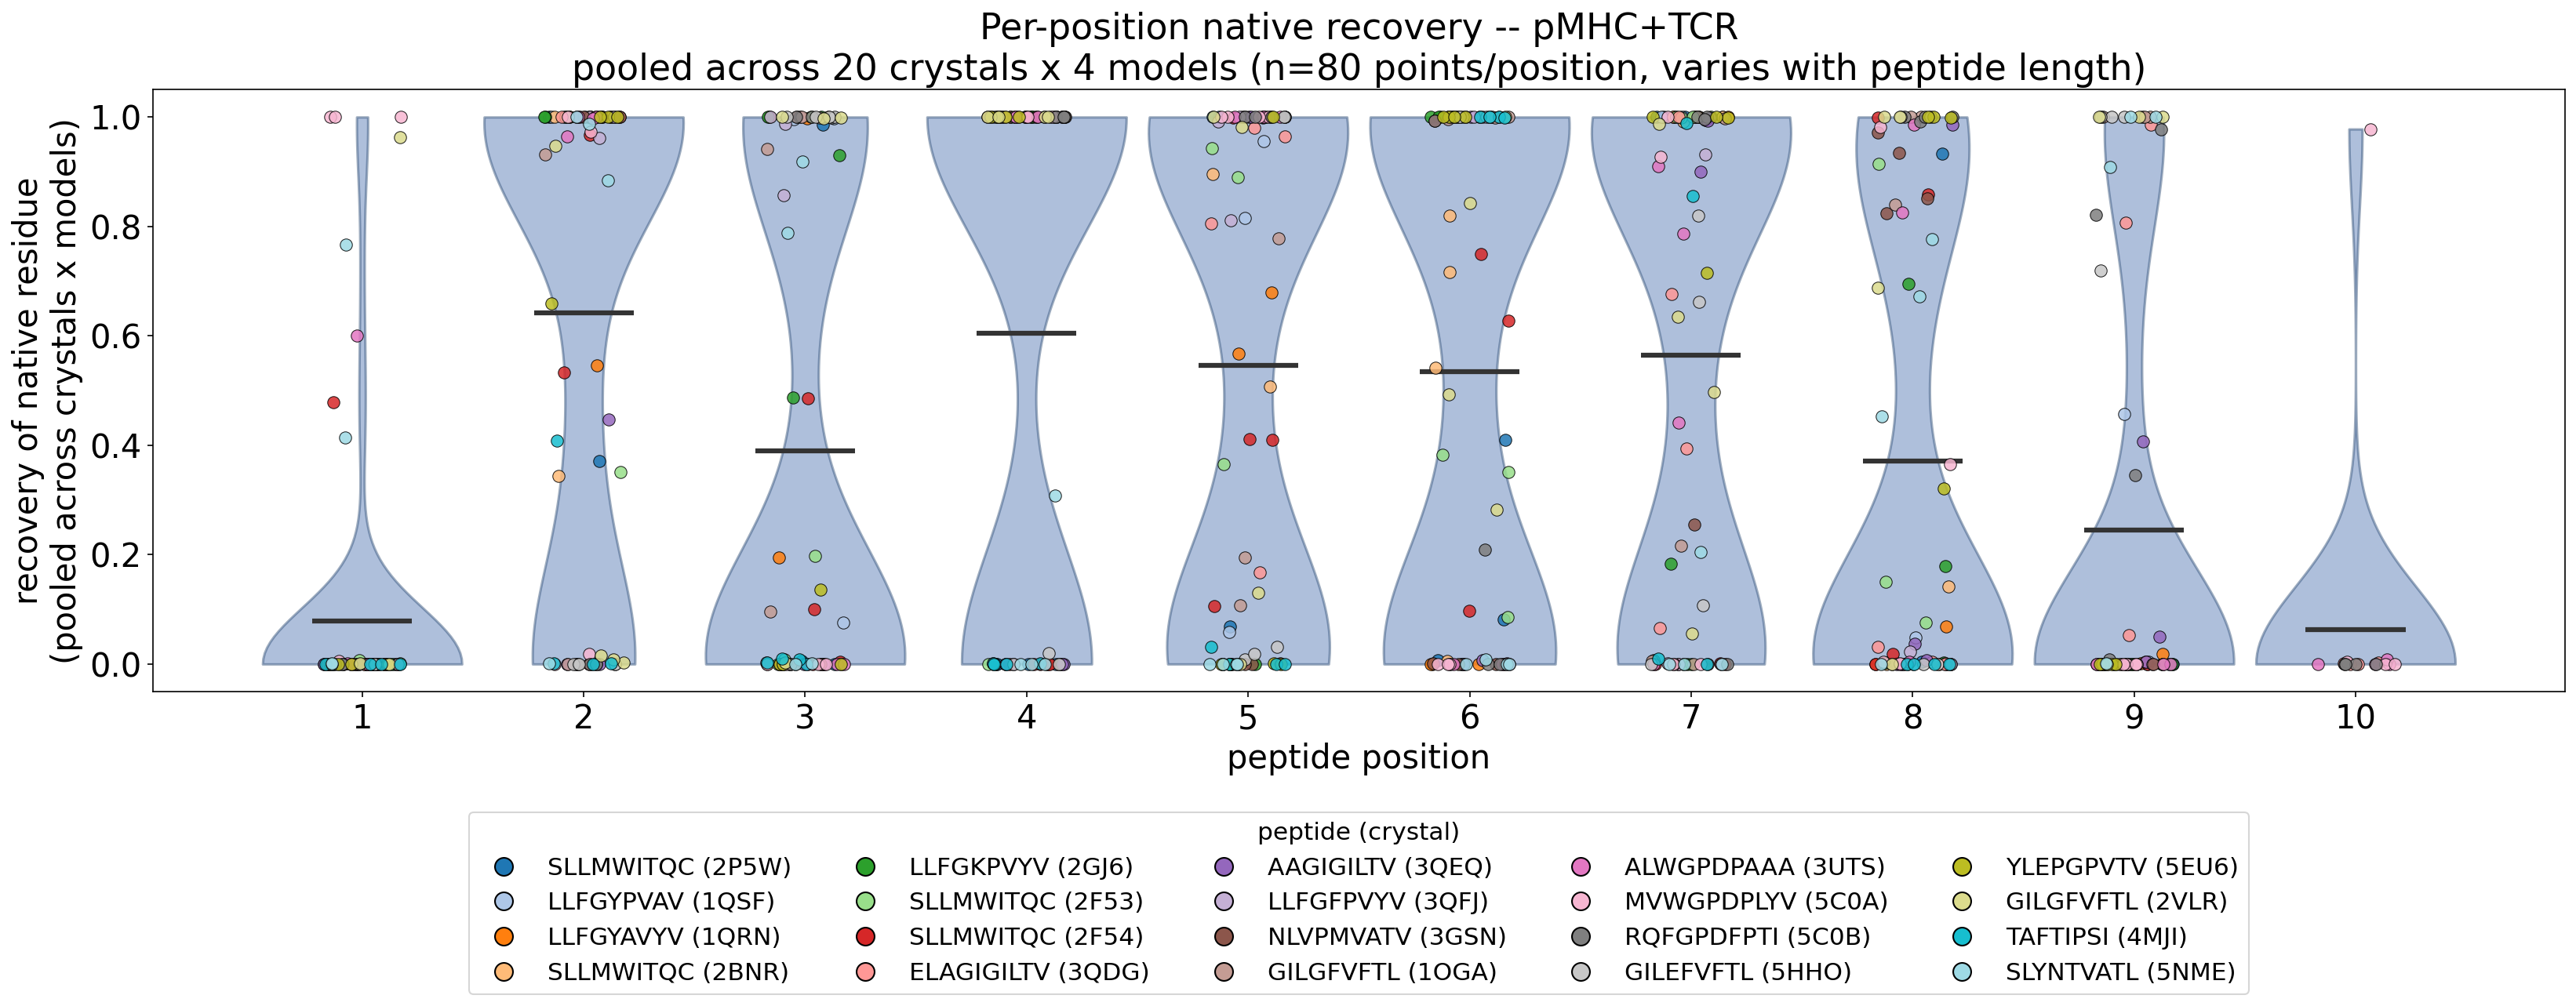
\includegraphics[width=\textwidth]{../figures/fig_panel3_recovery_presentation/fig_panel3_violin_summary_full.png}
\caption{\textbf{Per-position recovery is bimodal, and the two MHC anchors diverge.} Recovery
of the native residue, pooled across all 20 crystals and 4 models, one violin per peptide position
(pMHC+TCR context). Individual points are colored by crystal. P2 sits well above the interior average;
P$\Omega$ (the rightmost populated position for each peptide length) sits well below it; this is the
opposite of what "both are MHC anchors" would predict if anchoring alone determined recoverability.}
\label{fig:fig1}
\end{figure*}


Averaged across the entire peptide, the four models fall within a narrow band of mean recovery ($0.41$
to $0.47$ in full context and $0.28$ to $0.36$ without the TCR; Supplementary Figure~\ref{fig:supp5}),
narrow enough that the models might appear indistinguishable by inspection. A Friedman test indicates
otherwise in both contexts ($\chi^2=10.80$, $p=0.013$, full context; $\chi^2=12.18$, $p=0.007$, mhconly),
so this apparent similarity reflects proximity in magnitude rather than statistical equivalence. As an
aside, on 3QDG the central Gly-Ile-Gly motif at positions 4--6, well characterized in the literature,
recovers essentially perfectly here ($1.00$, $0.73$, $1.00$ vs.\ $0.49$), though we have not attempted a
systematic motif annotation across the full panel.

The relationship between resolution and recovery illustrates how pooling across a heterogeneous panel
can understate a genuine effect. Pooled across all twenty distinct peptides, the correlation is modest,
and only one model survives correction individually ($r=-0.49$ pooled, $p=0.030$; ESM-IF1 alone,
$r=-0.63$, $p=0.003$; Supplementary Figure~\ref{fig:supp6}). However, four of the twenty structures
(2P5W, 2BNR, 2F53, and 2F54) are independent crystals of the identical peptide (SLLMWITQC, the NY-ESO-1
epitope, a cancer-testis antigen widely targeted in adoptive T-cell and TCR-engineered immunotherapies)
bound to nearly the same TCR clone, differing primarily in resolution ($1.9$--$2.7$\,\AA). Holding
peptide identity fixed in this
way removes a confound that the pooled panel cannot, and the effect becomes unambiguous. Declining
resolution drives recovery down for two of the four models ($r=-0.99$, $p=0.012$, ProteinMPNN (no MHC);
$r=-0.97$, $p=0.031$, ESM-IF1) and drives unique design counts up for the remaining two ($r=0.97$,
$p=0.028$, ProteinMPNN; $r=0.96$, $p=0.040$, ProteinMPNN (no MHC); Supplementary Figure~\ref{fig:supp7}).
The pooled-panel estimate was therefore not incorrect, but diluted by heterogeneity.

\subsection{ProteinMPNN-Family Models Enrich for Predicted Strong pMHC Binders}
\label{sec:affinity}

Having established the recovery rates of the native peptide and the sequence space each structure
samples, we next asked whether those sampled peptides would actually be presented, scoring every unique
design from the nineteen HLA-A*02:01 structures for predicted HLA-A2 binding with two unrelated
predictors, MHCflurry and ESMCBA, neither of which had seen this panel (Figure~\ref{fig:fig2}).

\begin{figure*}[tb]
\centering
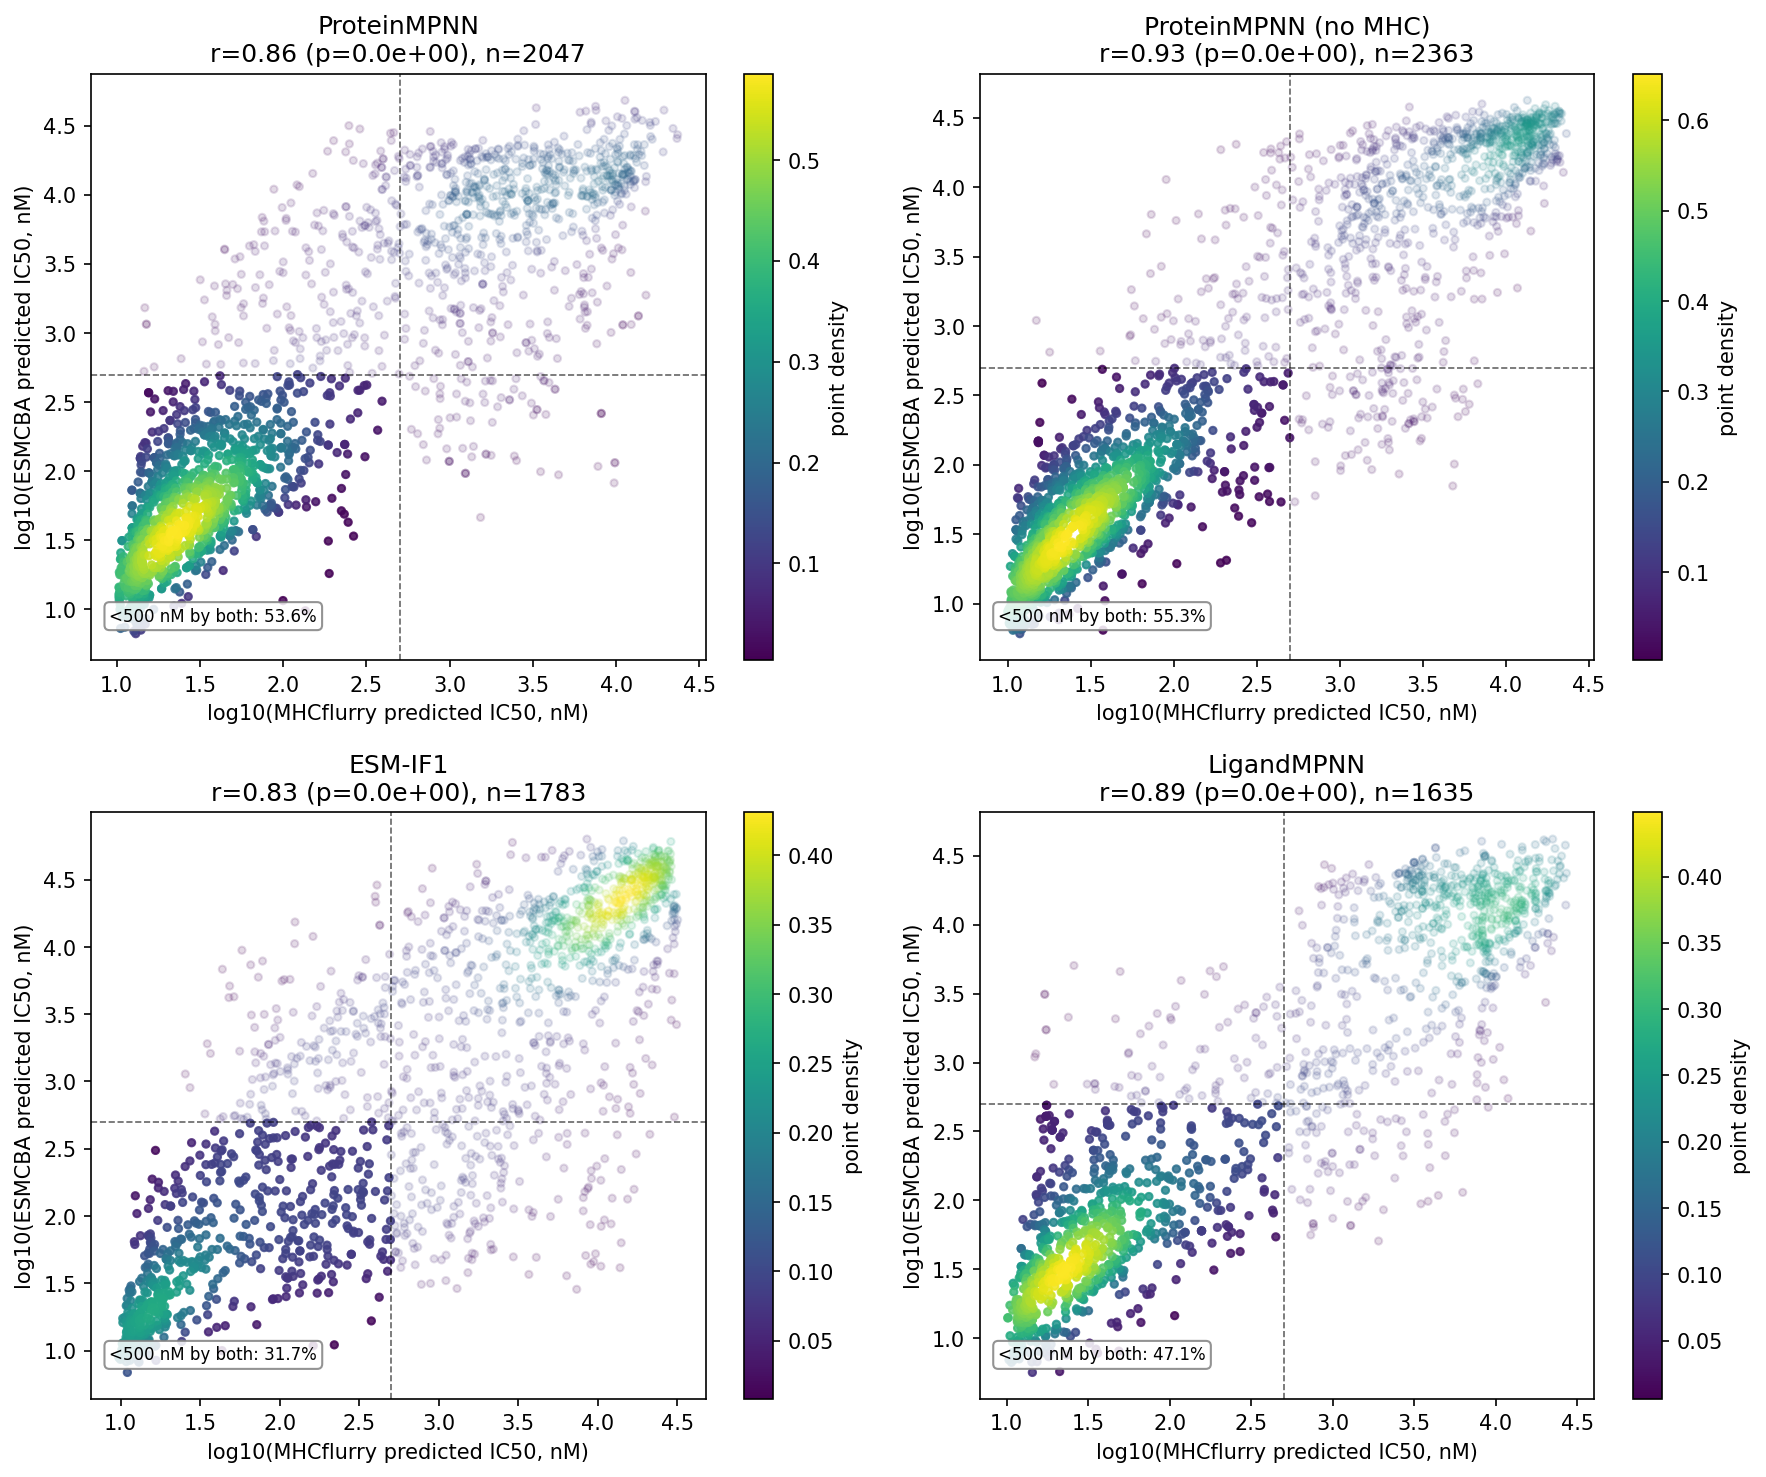
\includegraphics[width=\textwidth]{../figures/fig_panel6_mhcflurry_esmcba_umap/fig_panel6_esmcba_vs_mhcflurry_by_model.png}
\caption{\textbf{MHCflurry and ESMCBA agree closely on which designs bind tightly.} log10(predicted
IC50, nM) for both predictors, pMHC+TCR context, one panel per model. Dashed lines mark the 500\,nM
strong-binder cutoff on both axes; only designs strong by \emph{both} predictors jointly (bottom-left
quadrant) are rendered opaque, everything outside that quadrant is faded. The percentage is the joint
strong-binder rate, meaning the fraction of designs under 500\,nM by both predictors at once.}
\label{fig:fig2}
\end{figure*}

The two predictors agree closely on the same designs ($r=0.83$--$0.91$ per model in full context, up to
$0.94$ without the TCR), and agreement between two methodologically unrelated predictors constitutes
stronger evidence than either predictor alone. On this shared landscape, projected jointly into one UMAP
embedding space (Supplementary Figure~\ref{fig:supp11}), ProteinMPNN and LigandMPNN consistently sample
toward higher predicted affinity than ESM-IF1. At the 500\,nM cutoff, 61--78\% of ProteinMPNN-family and
LigandMPNN designs qualify by MHCflurry, compared with 45\% for ESM-IF1 ($\chi^2=238.46$,
$p=2\times10^{-51}$; see also Section~\ref{sec:tcr}). This pattern is better characterized as ESM-IF1 being a
consistent low-affinity outlier than as a general superiority of ProteinMPNN over ESM-IF1, since the
other three tools do not share this deficit.

\subsection{Removing the TCR Increases Diversity and Predicted Affinity, but Lowers Recovery}
\label{sec:tcr}

To understand the effect of the TCR on what these models propose, we resampled every structure with the
TCR deleted from the input and compared the resulting designs against the full-complex designs above.

Every model explores substantially more sequence space without the TCR, with unique design counts roughly
doubling or tripling (ProteinMPNN 1081 $\to$ 3671; ProteinMPNN (no MHC) 958 $\to$ 2362; ESM-IF1 1069 $\to$
1865; LigandMPNN 668 $\to$ 2111; Supplementary Figure~\ref{fig:supp5}). This larger space skews toward
higher predicted affinity, but not uniformly across models. ProteinMPNN (no MHC) shows the largest shift
(strong-binder rate 77.5\%$\to$95.2\%), LigandMPNN a smaller but genuine one ($61.1\%\to70.7\%$), while
ProteinMPNN and ESM-IF1 show little change (Supplementary Figure~\ref{fig:supp10}). The affinity gain
associated with TCR removal thus appears concentrated in the two models already most context-sensitive,
rather than reflecting a general consequence of removing the TCR.

A related but distinct signal comes from each model's own confidence in the sequences it designs,
independent of either external predictor. ProteinMPNN and ProteinMPNN (no MHC) report an average
per-residue negative log-likelihood for each design, for which lower values indicate higher confidence;
LigandMPNN reports an overall confidence score, for which higher values indicate higher confidence.
Pooled across all nineteen HLA-A*02:01 structures, removing the TCR shifts this internal score for every
model, and in every case toward lower self-assessed confidence (ProteinMPNN mean $1.016\to1.295$;
ProteinMPNN (no MHC) $0.925\to1.128$; LigandMPNN $0.413\to0.321$; Mann-Whitney $p<10^{-200}$ for all
three; Supplementary Figure~\ref{fig:supp9a}). This shift is not uniform across the panel. Broken out per
structure and Bonferroni-corrected, it reaches significance in 15--17 of 19 structures depending on the
model, but not in the remaining two to four (Supplementary Figure~\ref{fig:supp9b}). That a model can
become less confident in its own designs by its own internal metric while simultaneously being scored as
a stronger binder by an external predictor that never saw those designs indicates that the two signals
are not redundant, since one reflects how comfortably a sequence fits the model's learned distribution, the
other how likely it is to bind, and removing the TCR does not move them the same way. This distinction is
more informative than amino-acid-level recovery or composition alone, since it speaks to what the model
itself, not just an external predictor, "believes" about the sequences it is generating.

\subsection{Recovery Loss Concentrates at Experimentally Validated TCR-Contact Positions}
\label{sec:skempi}

To understand how these residue interactions contribute functionally to TCR binding, we tested whether
the recovery lost without the TCR concentrates at positions that experimental data already implicate in
receptor engagement. We cross-referenced SKEMPI 2.0 and IEDB against each structure's
crystallized TCR clone (matched by CDR3 sequence) and identified 21 (structure, position) pairs with an
experimentally measured mutation that alters TCR binding. Pooling recovery across exactly these
positions, TCR-present designs recover the native residue $54$--$58\%$ of the time, compared with
$34$--$38\%$ for TCR-absent designs (Figure~\ref{fig:fig3}), a consistent, though not universal, gap; a
minority of individual positions move in the opposite direction. The clearest single illustration lies
outside this panel, at position 4 of the MEL5/ELAGIGILTV complex, where SKEMPI confirms that alanine
substitution abolishes TCR binding outright, recovery in our data collapses from $98\%$ with the TCR to
$0\%$ without it.

\begin{figure*}[tb]
\centering
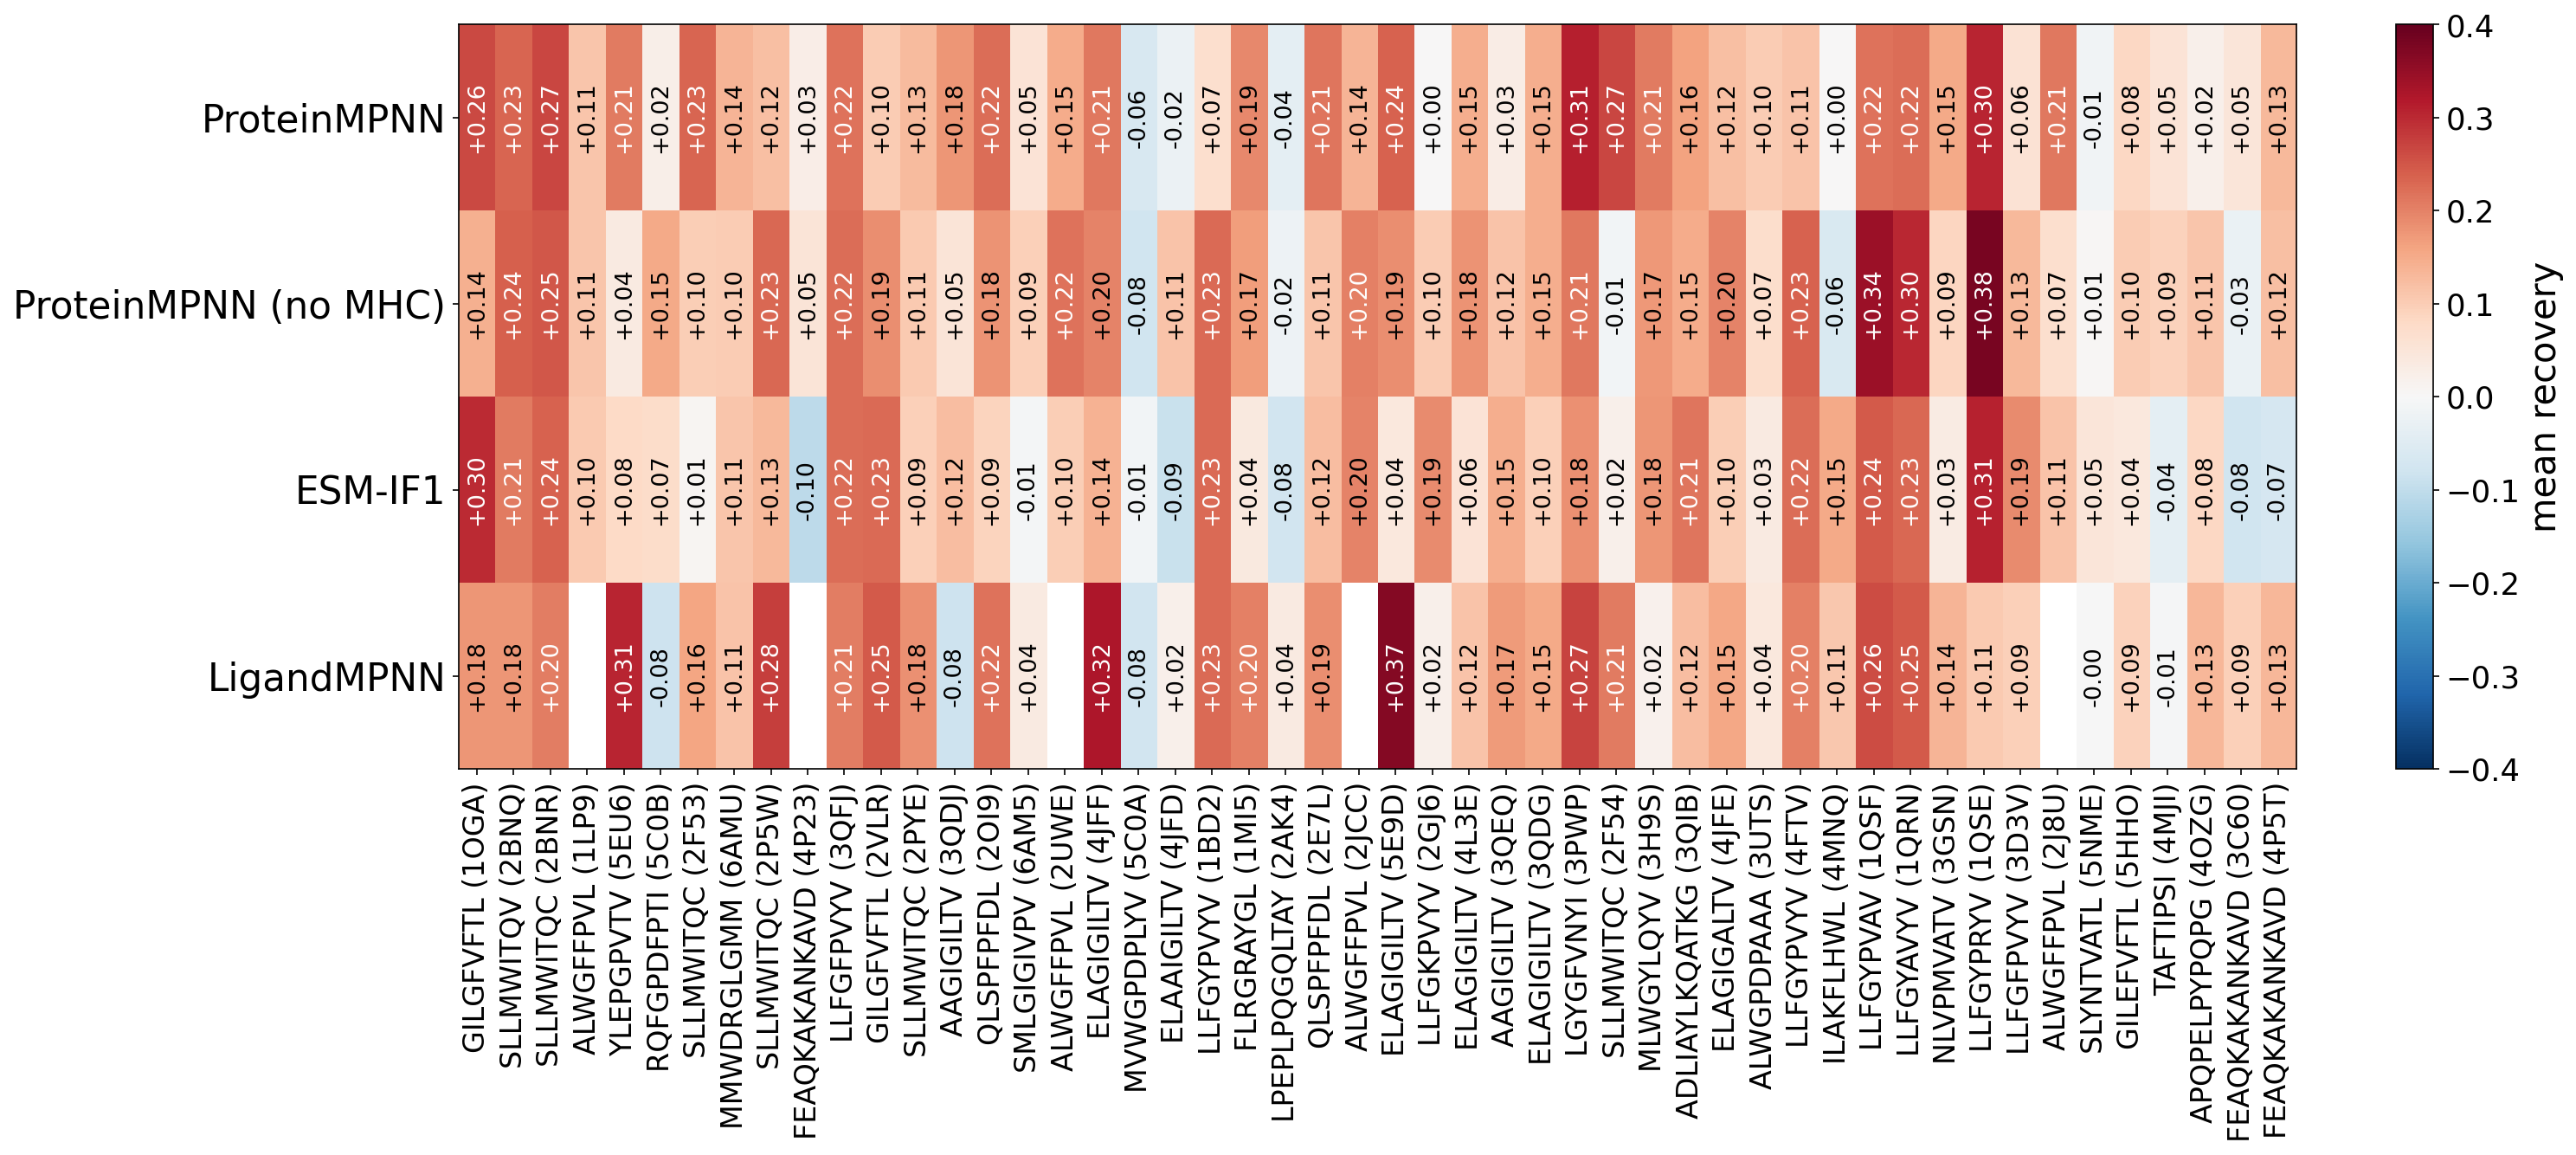
\includegraphics[width=0.85\textwidth]{../figures/fig_panel3_recovery_presentation/fig_panel3_delta_recovery_heatmap.png}
\caption{\textbf{Where the TCR-context benefit actually concentrates.} Recovery(full) $-$
recovery(mhconly), per crystal per model, crystals ordered by resolution (best to worst, left to right).
70 of 80 (model, crystal) cells are positive; mean $\Delta=+0.128$. The benefit is broad but not uniform,
and does not track resolution in any simple way.}
\label{fig:fig3}
\end{figure*}

\section{Discussion}

The unifying observation of this study is that the claim "MHC anchor positions matter" is true yet, on
its own, of limited explanatory value. P2 and P$\Omega$ are both structurally indispensable, yet behave
oppositely under inverse folding because one is a side-chain readout and the other is predominantly a
backbone constraint tolerant of many side chains. This distinction, rather than a blanket statement
about anchor positions, is what a sequence-design model can meaningfully report. The same caution
regarding pooled analyses applies to resolution, where a weak, borderline correlation pooled across twenty
distinct peptides conceals an unambiguous, model-specific effect once peptide identity is controlled for
using a same-peptide replicate set, the four independent SLLMWITQC/NY-ESO-1 crystals. The TCR-removal
results likewise resist a single summary verdict by
construction, since diversity increases for every model, affinity increases primarily for two of them, and
recovery decreases on average but not at every position, because "does the model require the TCR" was
never a single, unified question.

\section{Limitations and scope}
\label{sec:limitations}

\begin{itemize}
\item \textbf{$T{=}0.1$ only.}
\item \textbf{Allele skew.} Nineteen of twenty structures are HLA-A*02:01; the one exception (4MJI,
HLA-B*51:01) is also the hardest structure in the panel by recovery, and with $n=1$ we cannot separate
allele identity from TCR identity or structure-specific difficulty.
\item \textbf{Predicted affinity is not measured affinity.} Agreement between MHCflurry and ESMCBA
constitutes real evidence, but neither substitutes for an experimental binding assay.
\item \textbf{Not all TCR-binding evidence decouples MHC loading from TCR engagement equally well.} Only
SPR-based dissociation-constant measurements are performed on an already-folded pMHC complex; functional
assays (cytotoxicity, activation) cannot distinguish a peptide that ceased binding MHC from one that
ceased being recognized by the TCR.
\item \textbf{Recovery is not validated binding.} It measures agreement with a crystallized peptide, not
experimentally confirmed activity of the designed sequences.
\item \textbf{The MEL5/ELAGIGILTV case study is outside the 20-structure panel} and uses a separate,
earlier design campaign; it's a sharper single-structure illustration, not panel-scale evidence.
\end{itemize}

\section{Data and code availability}
\label{sec:data}

All data and code are available in the if-mhc GitHub repository:
\url{https://github.com/sermare/if-mhc}.

\FloatBarrier
\appendix
\section{Supplementary Figures}

\begin{table*}[p]
\renewcommand{\thetable}{S1}
\centering
\small
\begin{tabular}{@{}lcp{4.2cm}p{5.2cm}p{2.6cm}@{}}
\toprule
Model & Params & Architecture & Training data & Predicted structures \\
\midrule
ProteinMPNN & 1.66M & Message-passing GNN & PDB (\texttt{pdb\_2021aug02}), general backbones & -- \\[2pt]
ProteinMPNN (no MHC) & 1.66M & Message-passing GNN (identical to above) & Same corpus, MHC/TCR-class structures excluded & -- \\[2pt]
ESM-IF1 & 141.7M & GVP-GNN + transformer & CATH-derived backbones & +12M AF2 structures \\[2pt]
LigandMPNN & 2.62M & Message-passing GNN + ligand context & PDB, augmented with explicit ligand/heteroatom context & -- \\
\bottomrule
\end{tabular}
\caption{\textbf{Models compared.} Parameter counts verified directly from each
checkpoint's \texttt{state\_dict}. ESM-IF1 is the only tool whose training set is built substantially
from AlphaFold2-predicted structures rather than solved crystal structures ($\sim$12M predicted backbones,
on top of its CATH-derived crystal set).}
\label{tab:models}
\end{table*}

\begin{table*}[p]
\renewcommand{\thetable}{S2}
\centering
\small
\begin{tabular}{lllll}
\toprule
PDB & Peptide & Length & Allele & Resolution (\AA) \\
\midrule
2P5W & SLLMWITQC & 9 & HLA-A*02:01 & 2.20 \\
1QSF & LLFGYPVAV & 9 & HLA-A*02:01 & 2.80 \\
1QRN & LLFGYAVYV & 9 & HLA-A*02:01 & 2.80 \\
2BNR & SLLMWITQC & 9 & HLA-A*02:01 & 1.90 \\
2GJ6 & LLFGKPVYV & 9 & HLA-A*02:01 & 2.56 \\
2F53 & SLLMWITQC & 9 & HLA-A*02:01 & 2.10 \\
2F54 & SLLMWITQC & 9 & HLA-A*02:01 & 2.70 \\
3QDG & ELAGIGILTV & 10 & HLA-A*02:01 & 2.69 \\
3QEQ & AAGIGILTV & 9 & HLA-A*02:01 & 2.59 \\
3QFJ & LLFGFPVYV & 9 & HLA-A*02:01 & 2.29 \\
3GSN & NLVPMVATV & 9 & HLA-A*02:01 & 2.80 \\
1OGA & GILGFVFTL & 9 & HLA-A*02:01 & 1.40 \\
3UTS & ALWGPDPAAA & 10 & HLA-A*02:01 & 2.71 \\
5C0A & MVWGPDPLYV & 10 & HLA-A*02:01 & 2.46 \\
5C0B & RQFGPDFPTI & 10 & HLA-A*02:01 & 2.03 \\
5HHO & GILEFVFTL & 9 & HLA-A*02:01 & 2.95 \\
5EU6 & YLEPGPVTV & 9 & HLA-A*02:01 & 2.02 \\
2VLR & GILGFVFTL & 9 & HLA-A*02:01 & 2.30 \\
4MJI & TAFTIPSI & 8 & HLA-B*51:01 & 2.99 \\
5NME & SLYNTVATL & 9 & HLA-A*02:01 & 2.94 \\
\bottomrule
\end{tabular}
\caption{\textbf{The twenty-structure panel.} PDB accession, native peptide,
peptide length, MHC allele, and crystallographic resolution for every structure in the panel.}
\label{tab:pdblist}
\end{table*}

\begin{figure*}[p]
\renewcommand{\thefigure}{S1a}
\centering
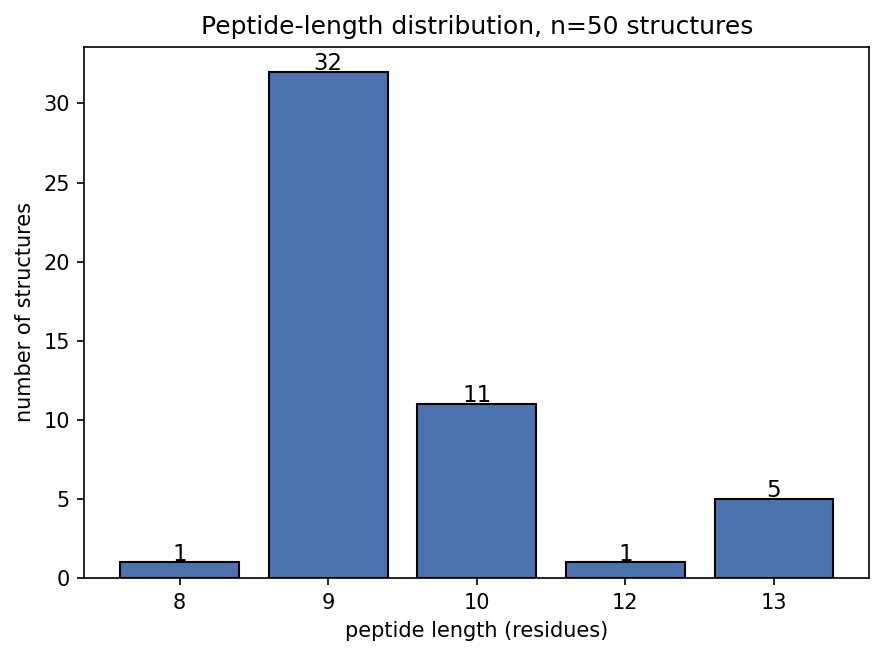
\includegraphics[width=0.75\textwidth]{../figures/fig_panel1_dataset_presentation/fig_panel1_peptide_length_dist.png}
\caption{\textbf{Peptide length distribution} across all 20 structures in the
panel.}
\label{fig:supp1a}
\end{figure*}

\begin{figure*}[p]
\renewcommand{\thefigure}{S1b}
\centering
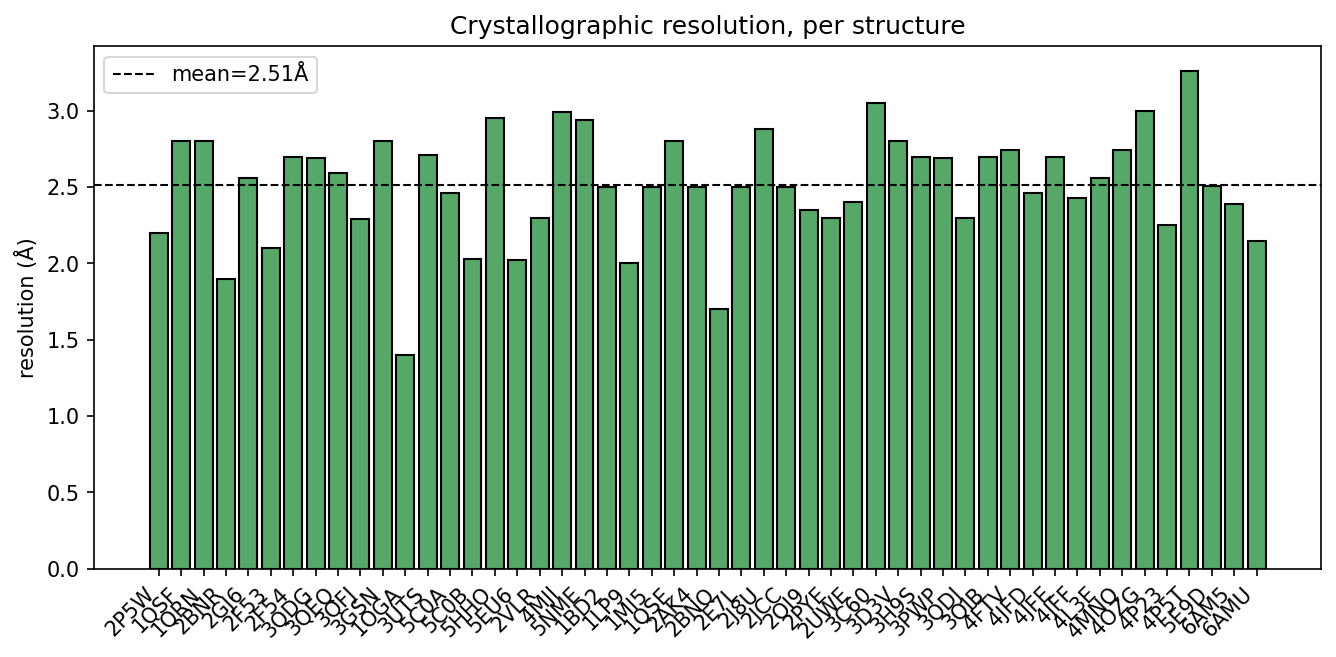
\includegraphics[width=0.75\textwidth]{../figures/fig_panel1_dataset_presentation/fig_panel1_resolution_dist.png}
\caption{\textbf{Crystallographic resolution per structure.}}
\label{fig:supp1b}
\end{figure*}

\begin{figure*}[p]
\renewcommand{\thefigure}{S1c}
\centering
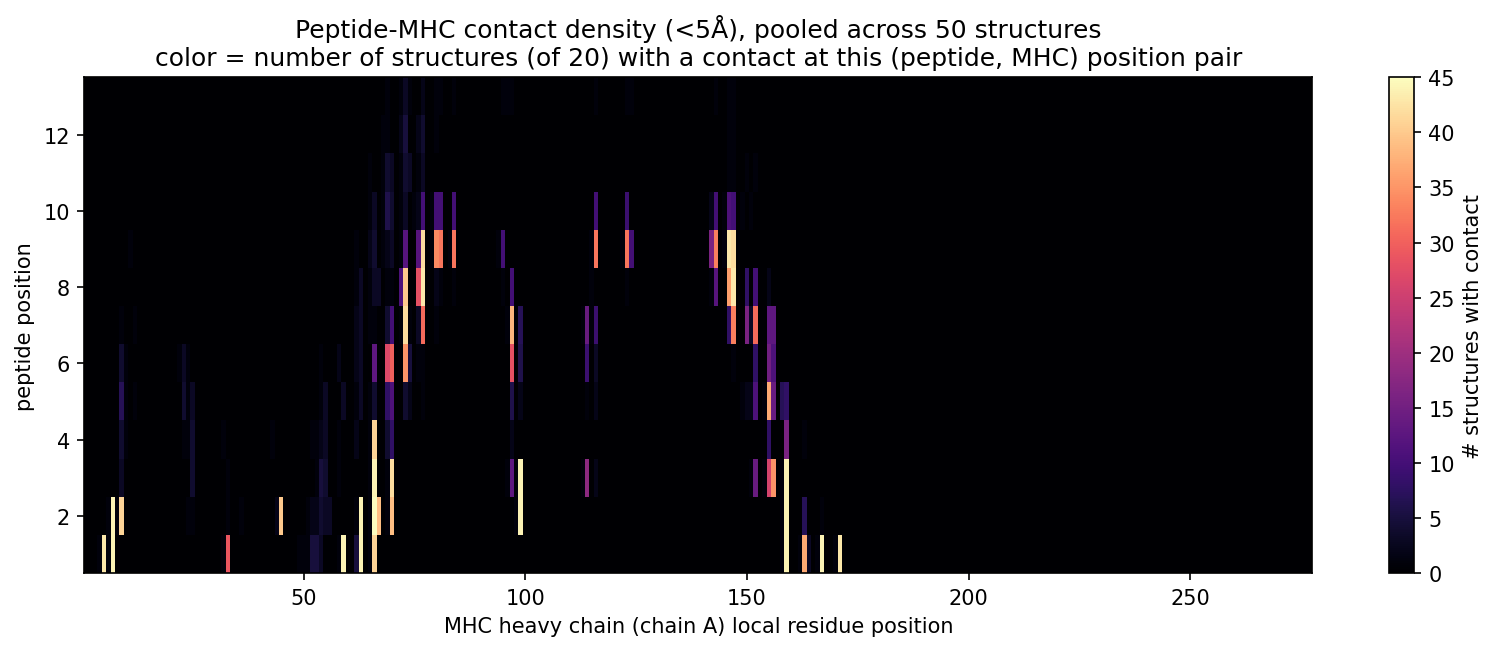
\includegraphics[width=0.75\textwidth]{../figures/fig_panel1_dataset_presentation/fig_panel1_mhc_contact_density.png}
\caption{\textbf{MHC residue vs.\ peptide contact density,} pooled across all
20 structures.}
\label{fig:supp1c}
\end{figure*}

\begin{figure*}[p]
\renewcommand{\thefigure}{S2}
\centering
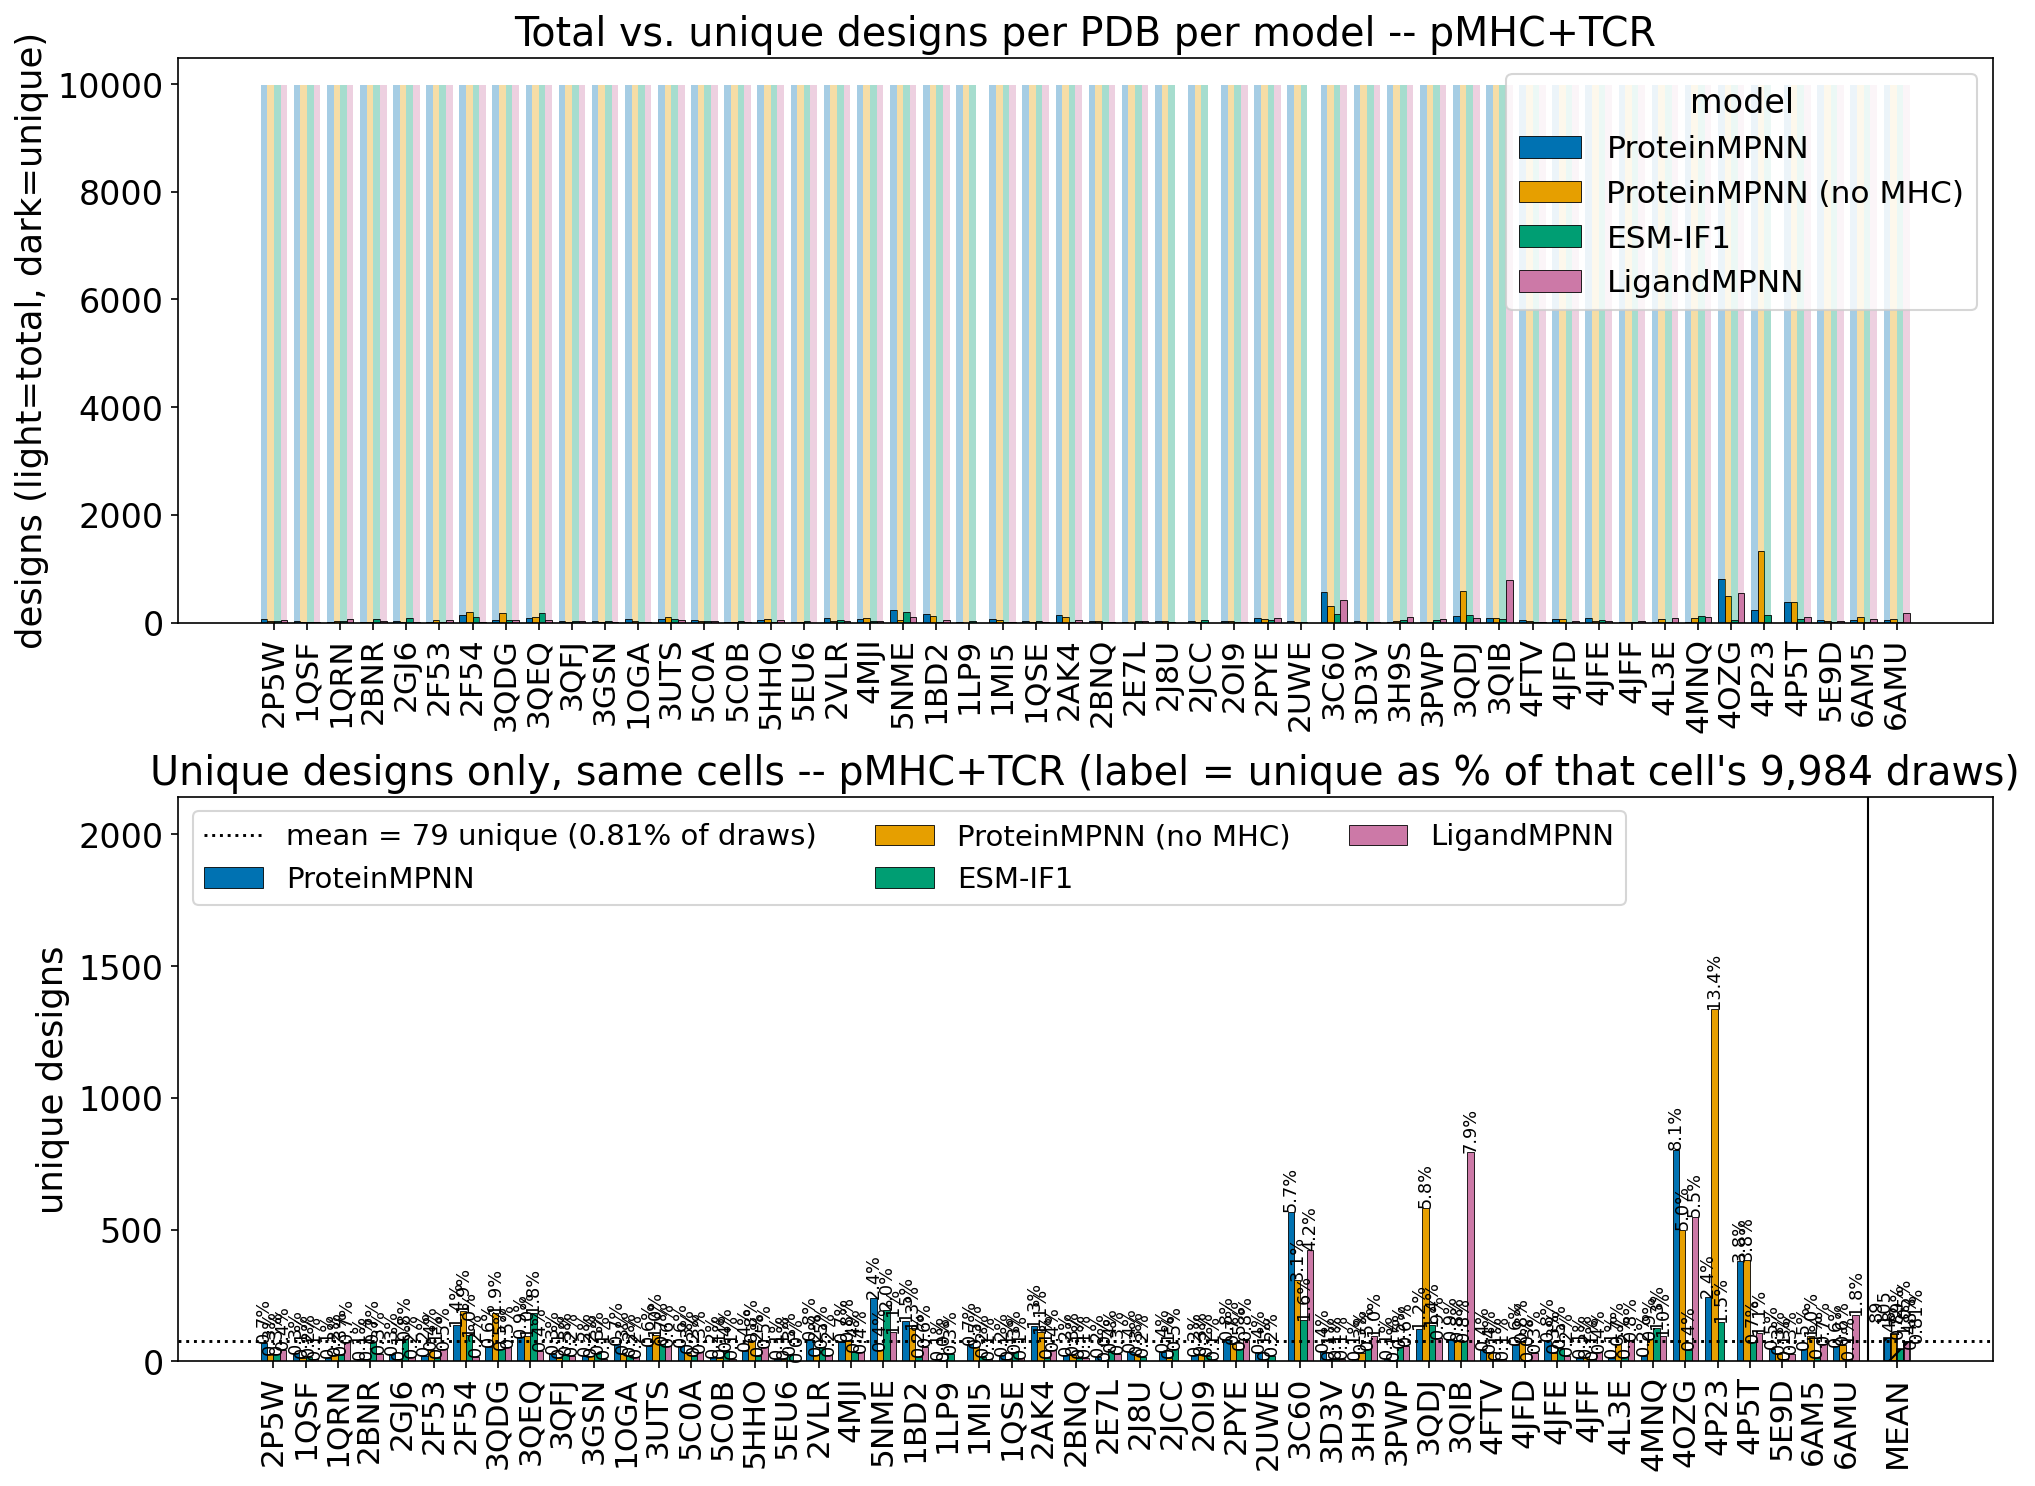
\includegraphics[width=0.85\textwidth]{../figures/fig_panel2_design_presentation/fig_panel2_total_vs_unique_full.png}
\caption{\textbf{Extreme redundancy at $T{=}0.1$.} 10,000 raw draws per
(structure, model); the unique fraction is $0.50\%$ on average and never exceeds a few percent.}
\label{fig:supp2}
\end{figure*}

\begin{figure*}[p]
\renewcommand{\thefigure}{S3}
\centering
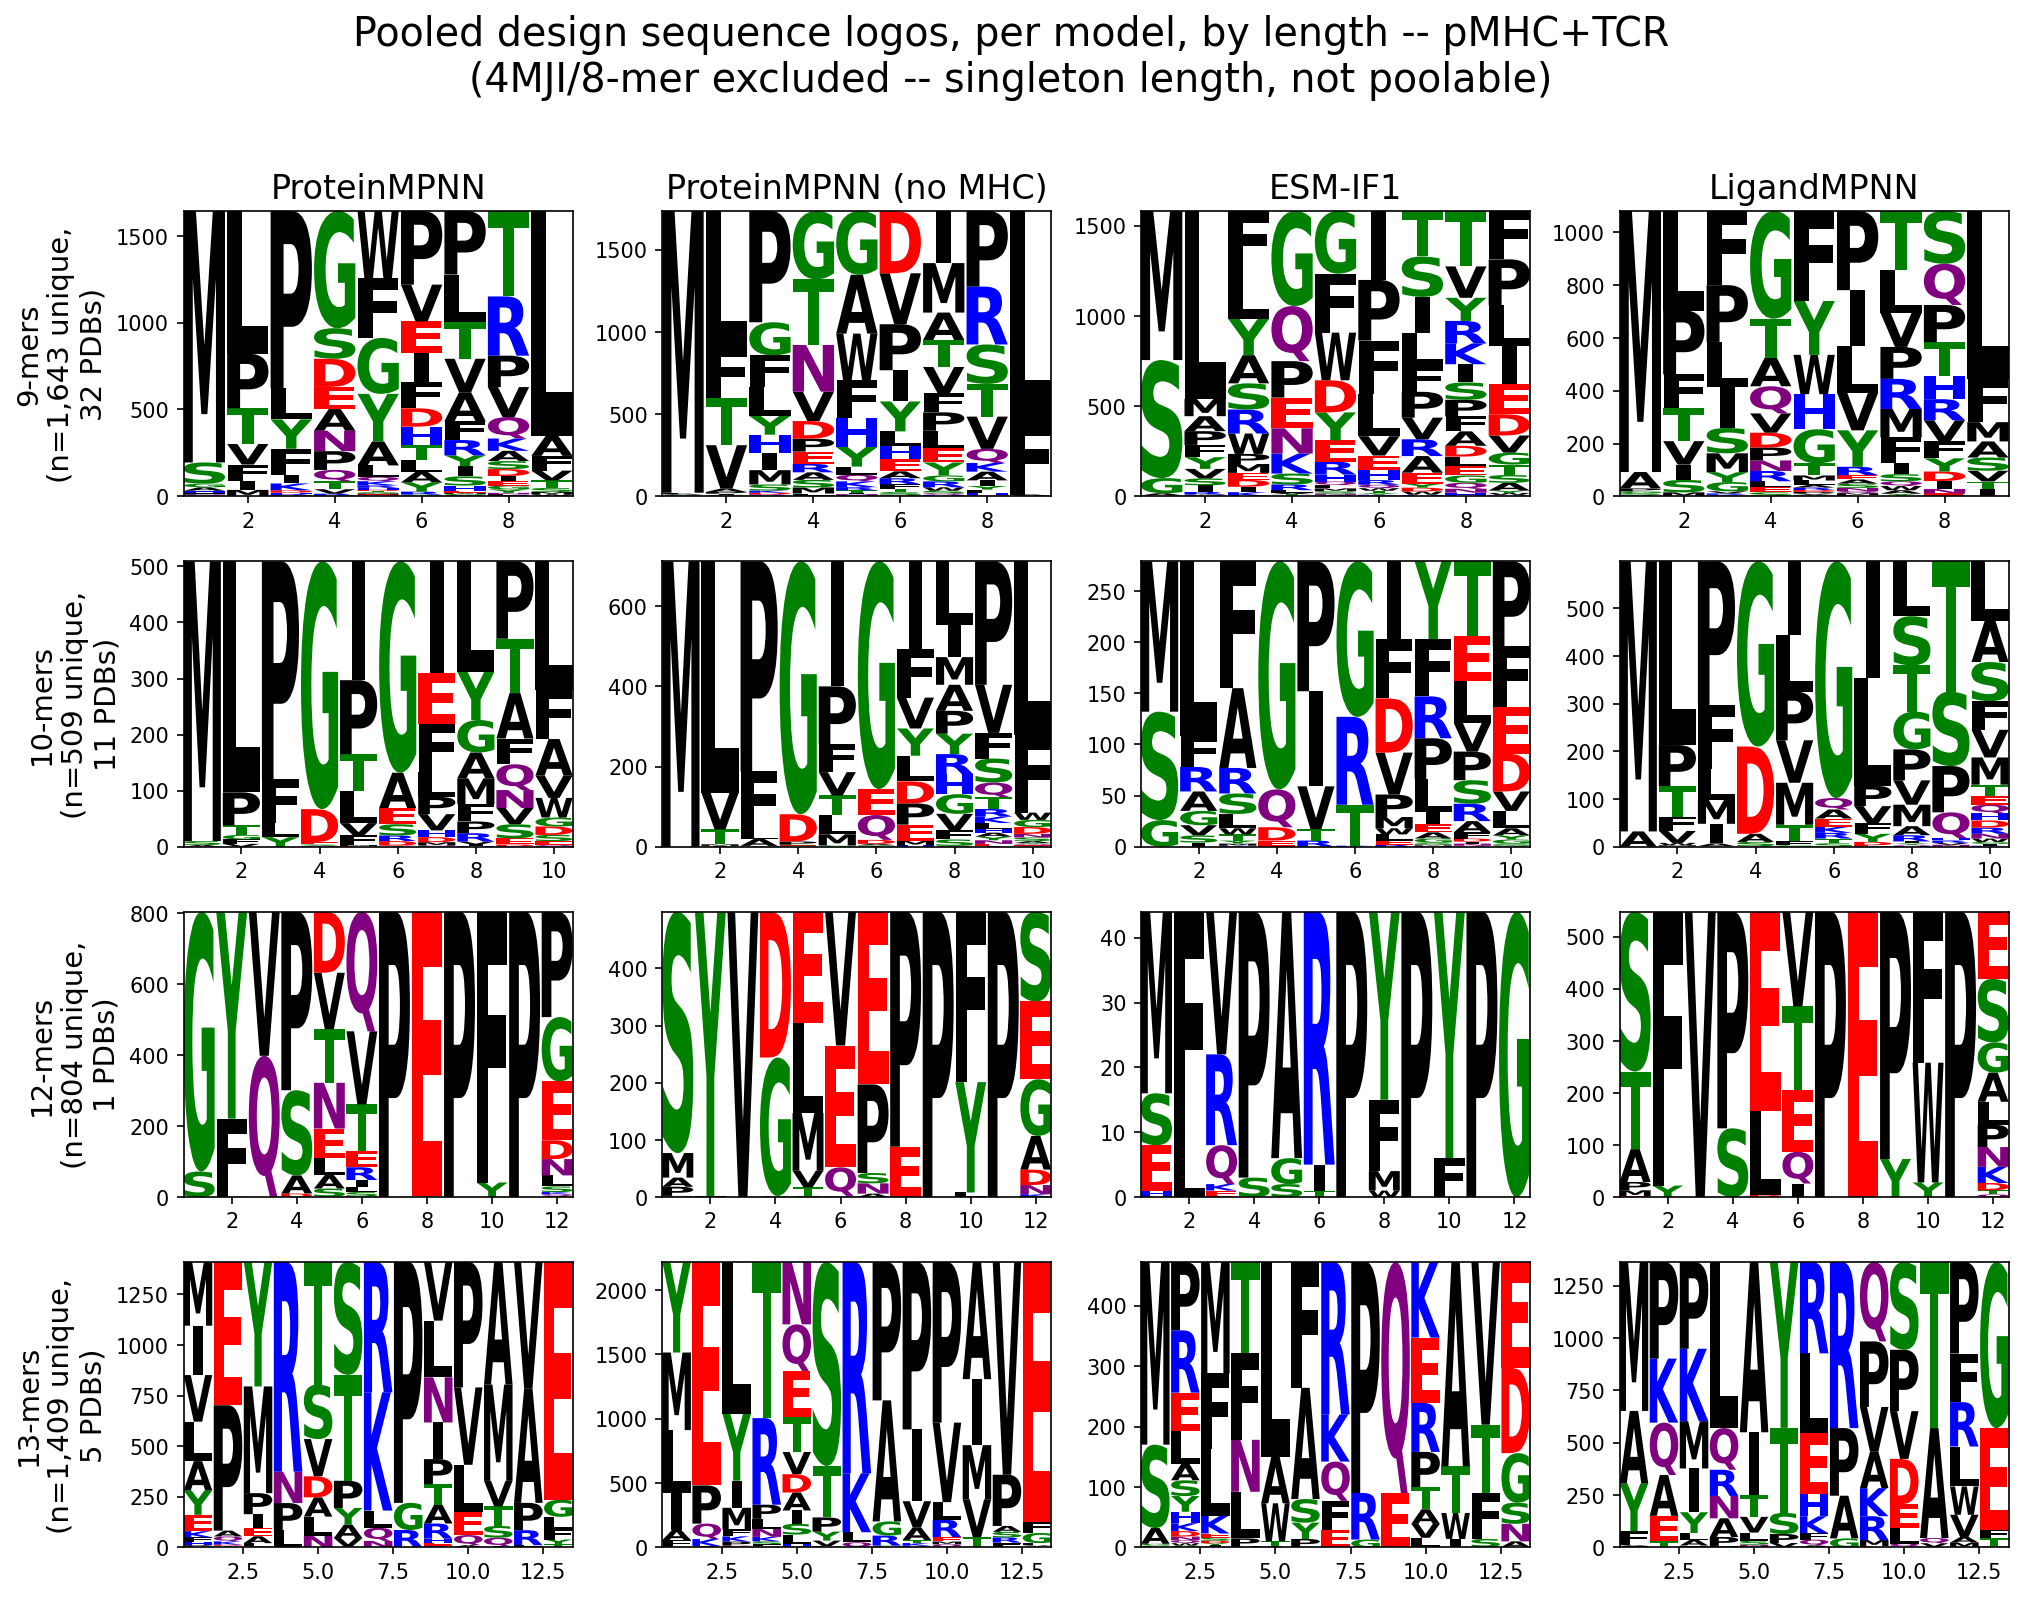
\includegraphics[width=0.85\textwidth]{../figures/fig_panel2_design_presentation/fig_panel2_design_logos_full.png}
\caption{\textbf{Design sequence logos, pooled by peptide length, one column per
model.}}
\label{fig:supp3}
\end{figure*}

\begin{figure*}[p]
\renewcommand{\thefigure}{S4a}
\centering
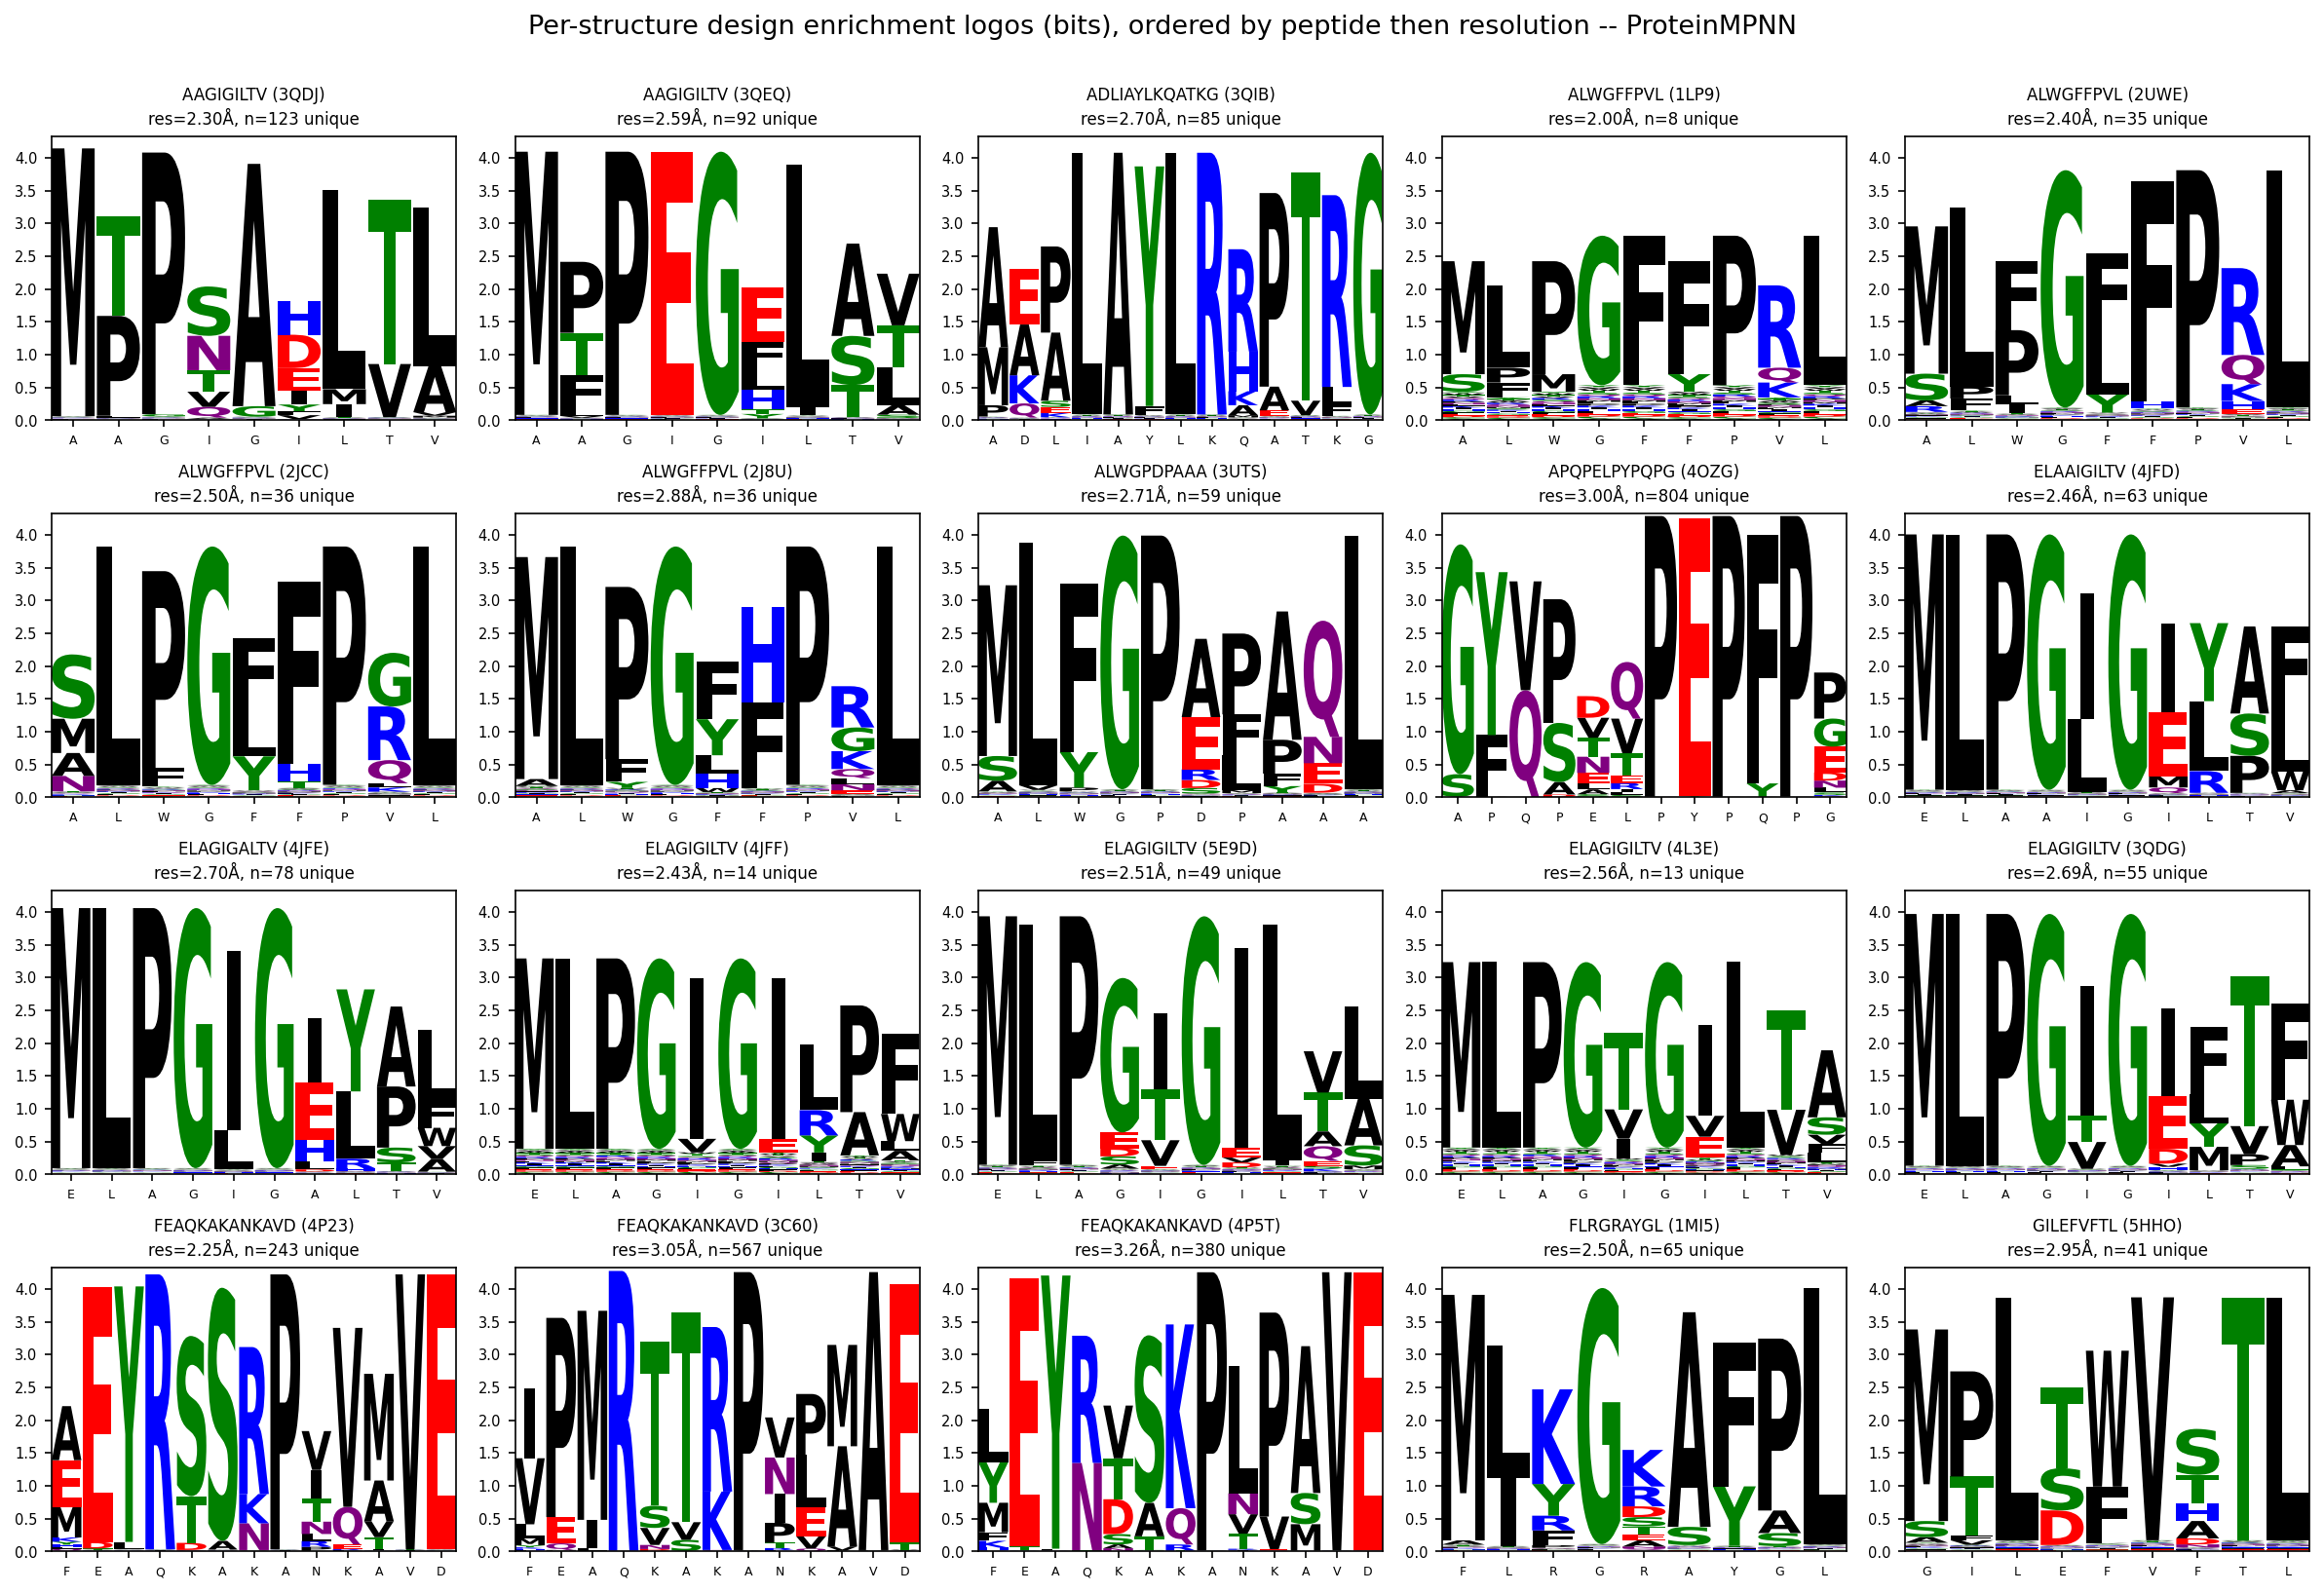
\includegraphics[width=0.7\textwidth]{../figures/fig_panel2_design_presentation/fig_panel2_design_logo_grid_vanilla.png}
\caption{\textbf{Per-structure design logos, ProteinMPNN.} All 20 structures,
ordered by native peptide then resolution.}
\label{fig:supp4a}
\end{figure*}

\begin{figure*}[p]
\renewcommand{\thefigure}{S4b}
\centering
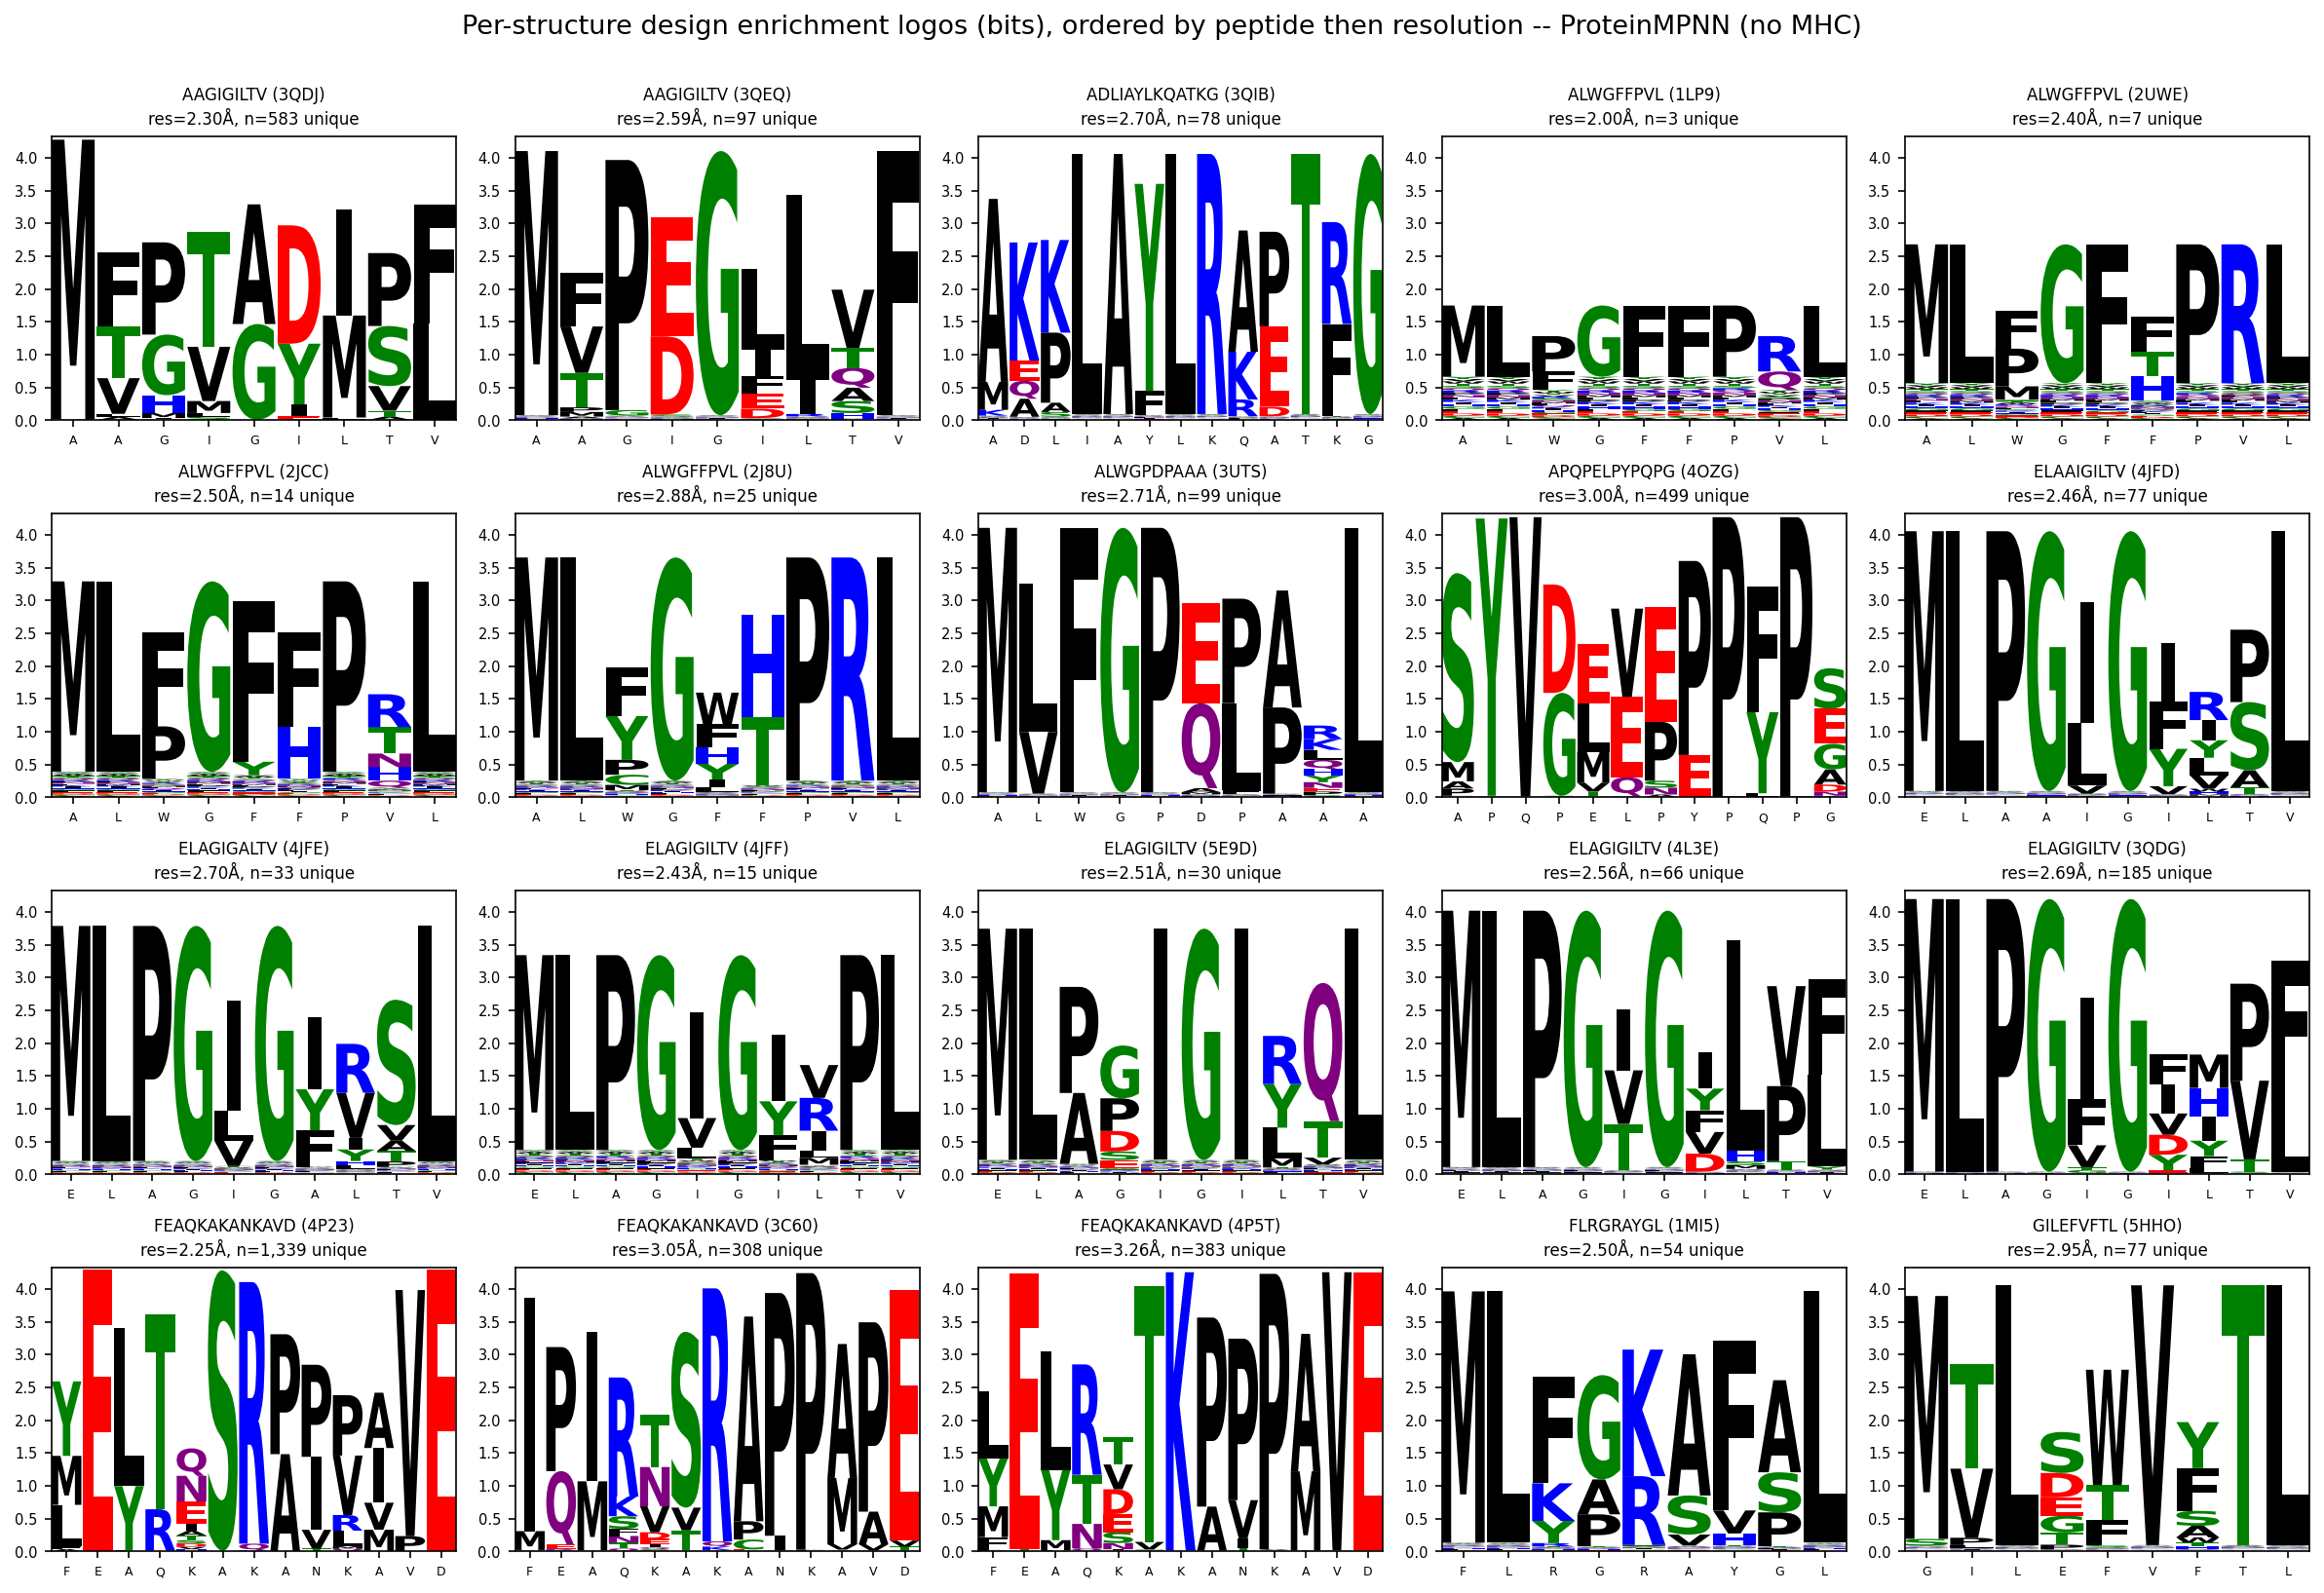
\includegraphics[width=0.7\textwidth]{../figures/fig_panel2_design_presentation/fig_panel2_design_logo_grid_noMHC.png}
\caption{\textbf{Per-structure design logos, ProteinMPNN (no MHC).}}
\label{fig:supp4b}
\end{figure*}

\begin{figure*}[p]
\renewcommand{\thefigure}{S4c}
\centering
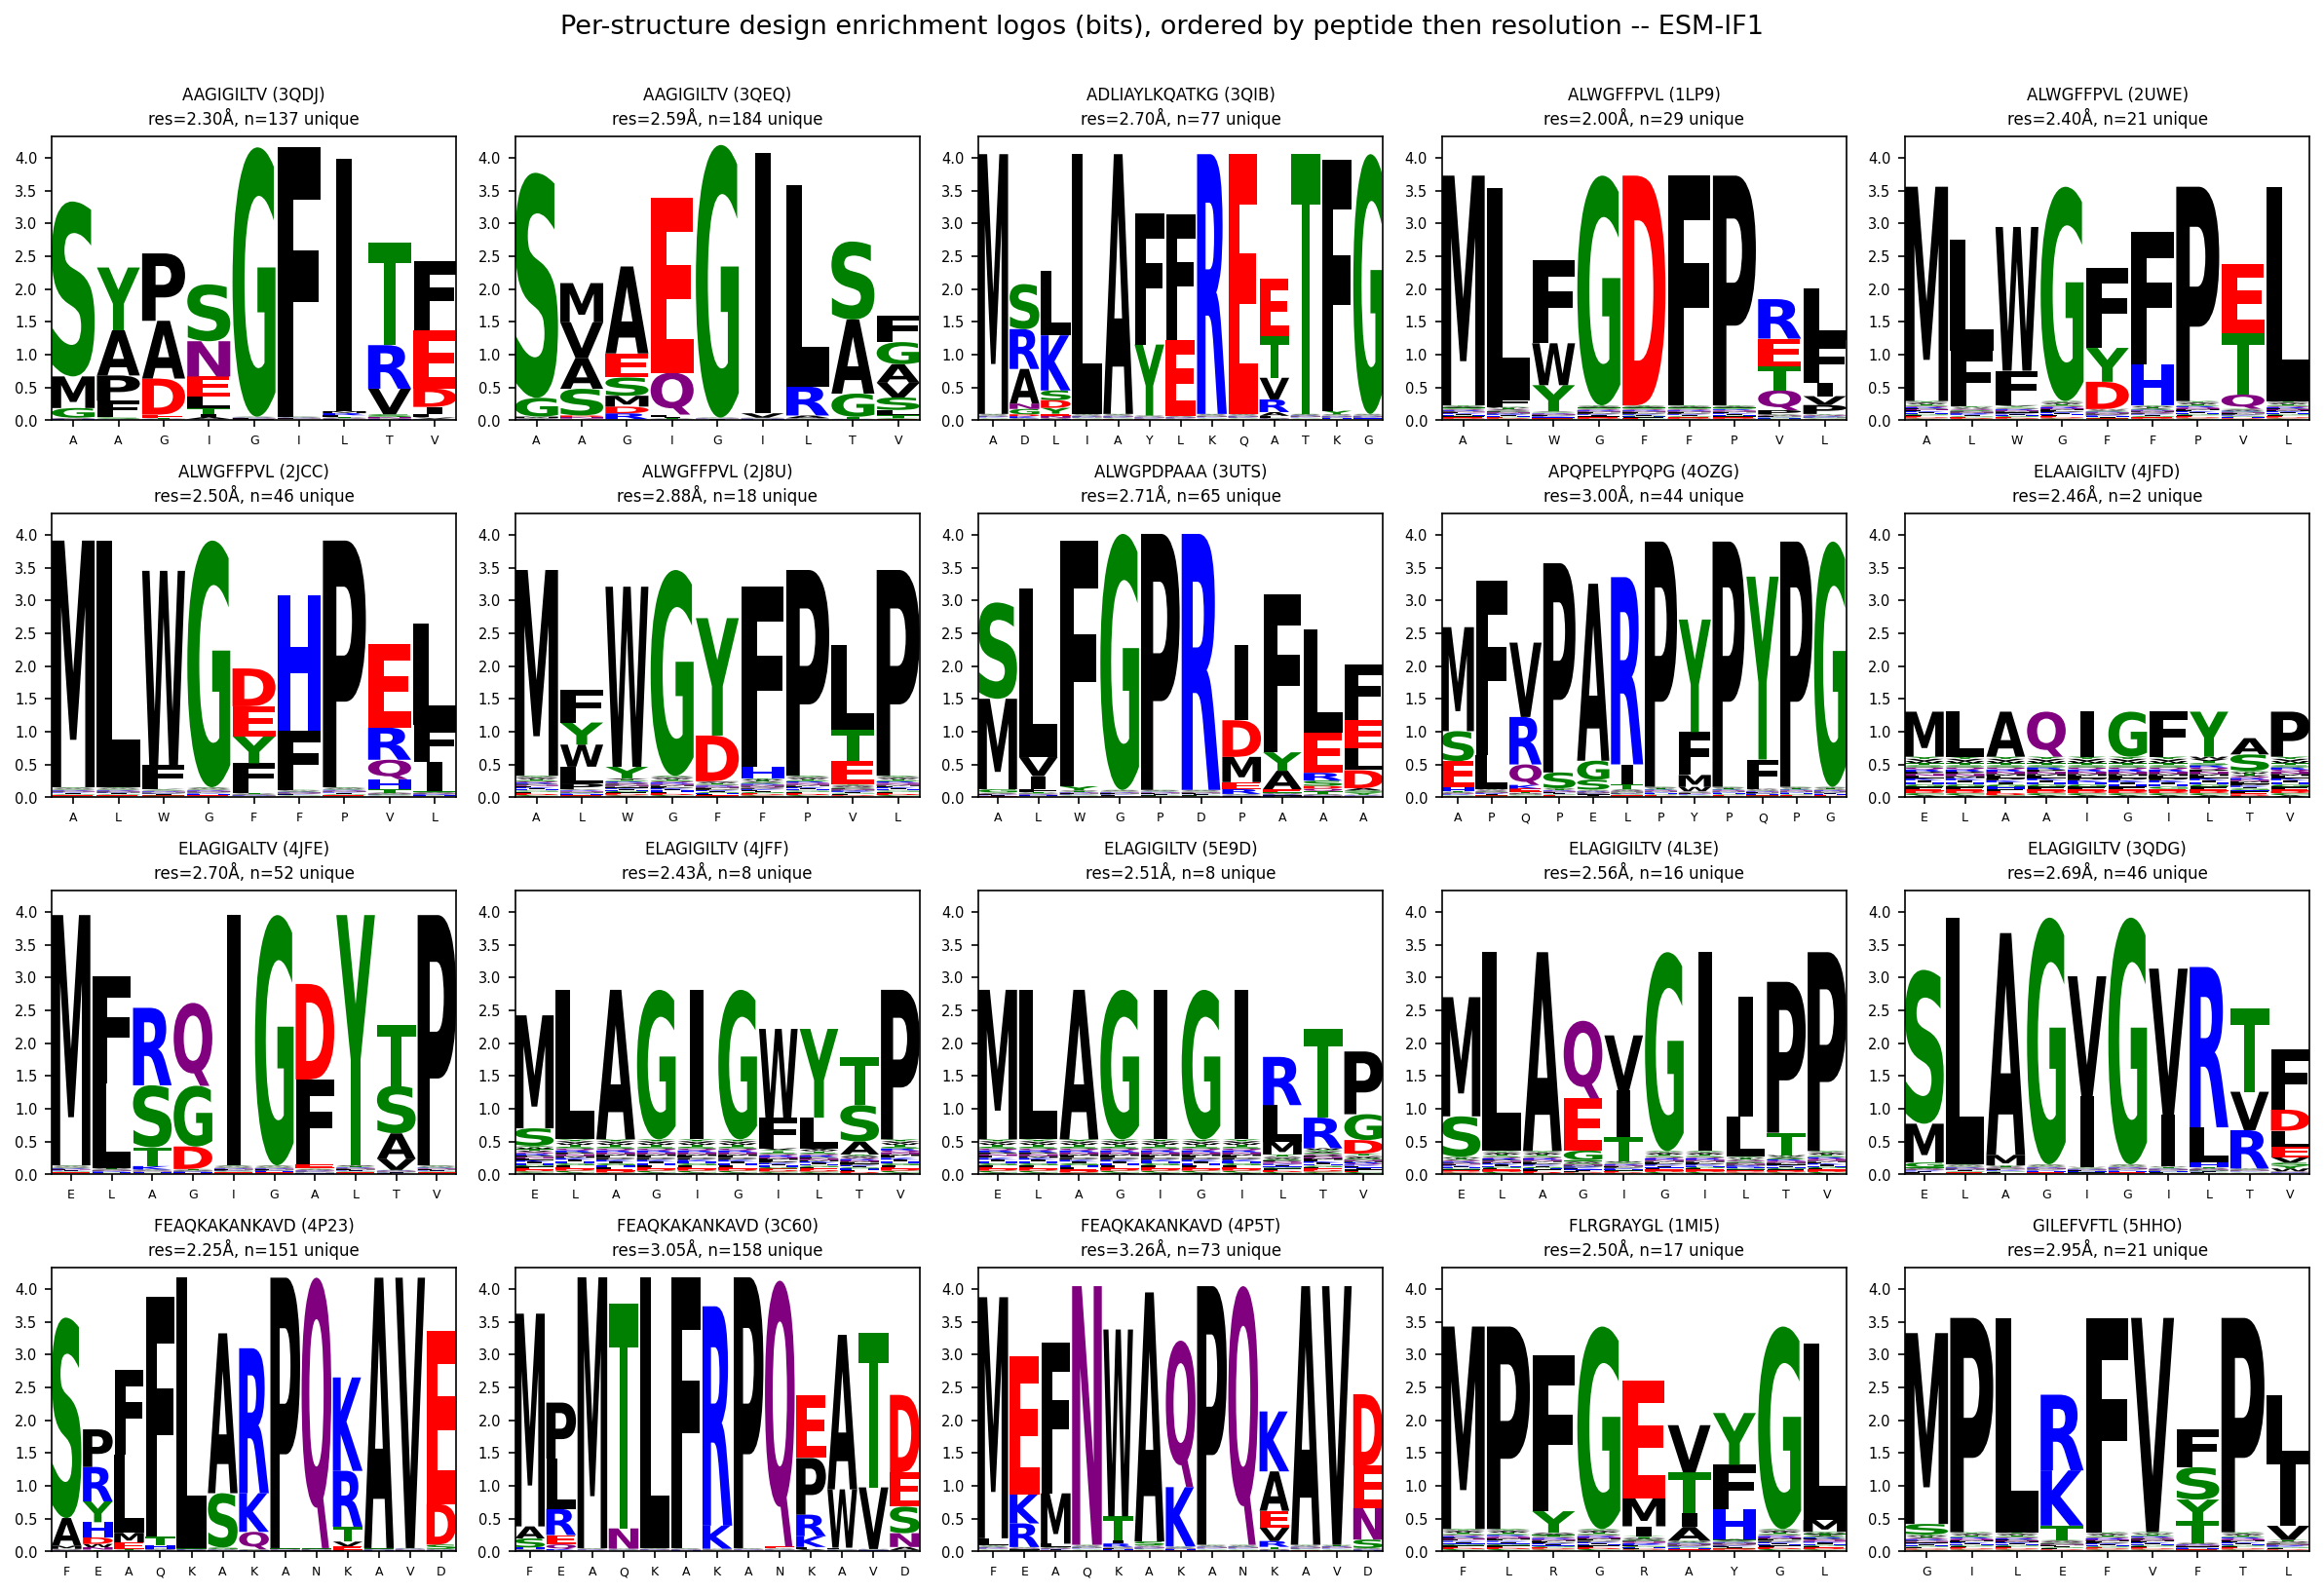
\includegraphics[width=0.7\textwidth]{../figures/fig_panel2_design_presentation/fig_panel2_design_logo_grid_ESM-IF1.png}
\caption{\textbf{Per-structure design logos, ESM-IF1.}}
\label{fig:supp4c}
\end{figure*}

\begin{figure*}[p]
\renewcommand{\thefigure}{S4d}
\centering
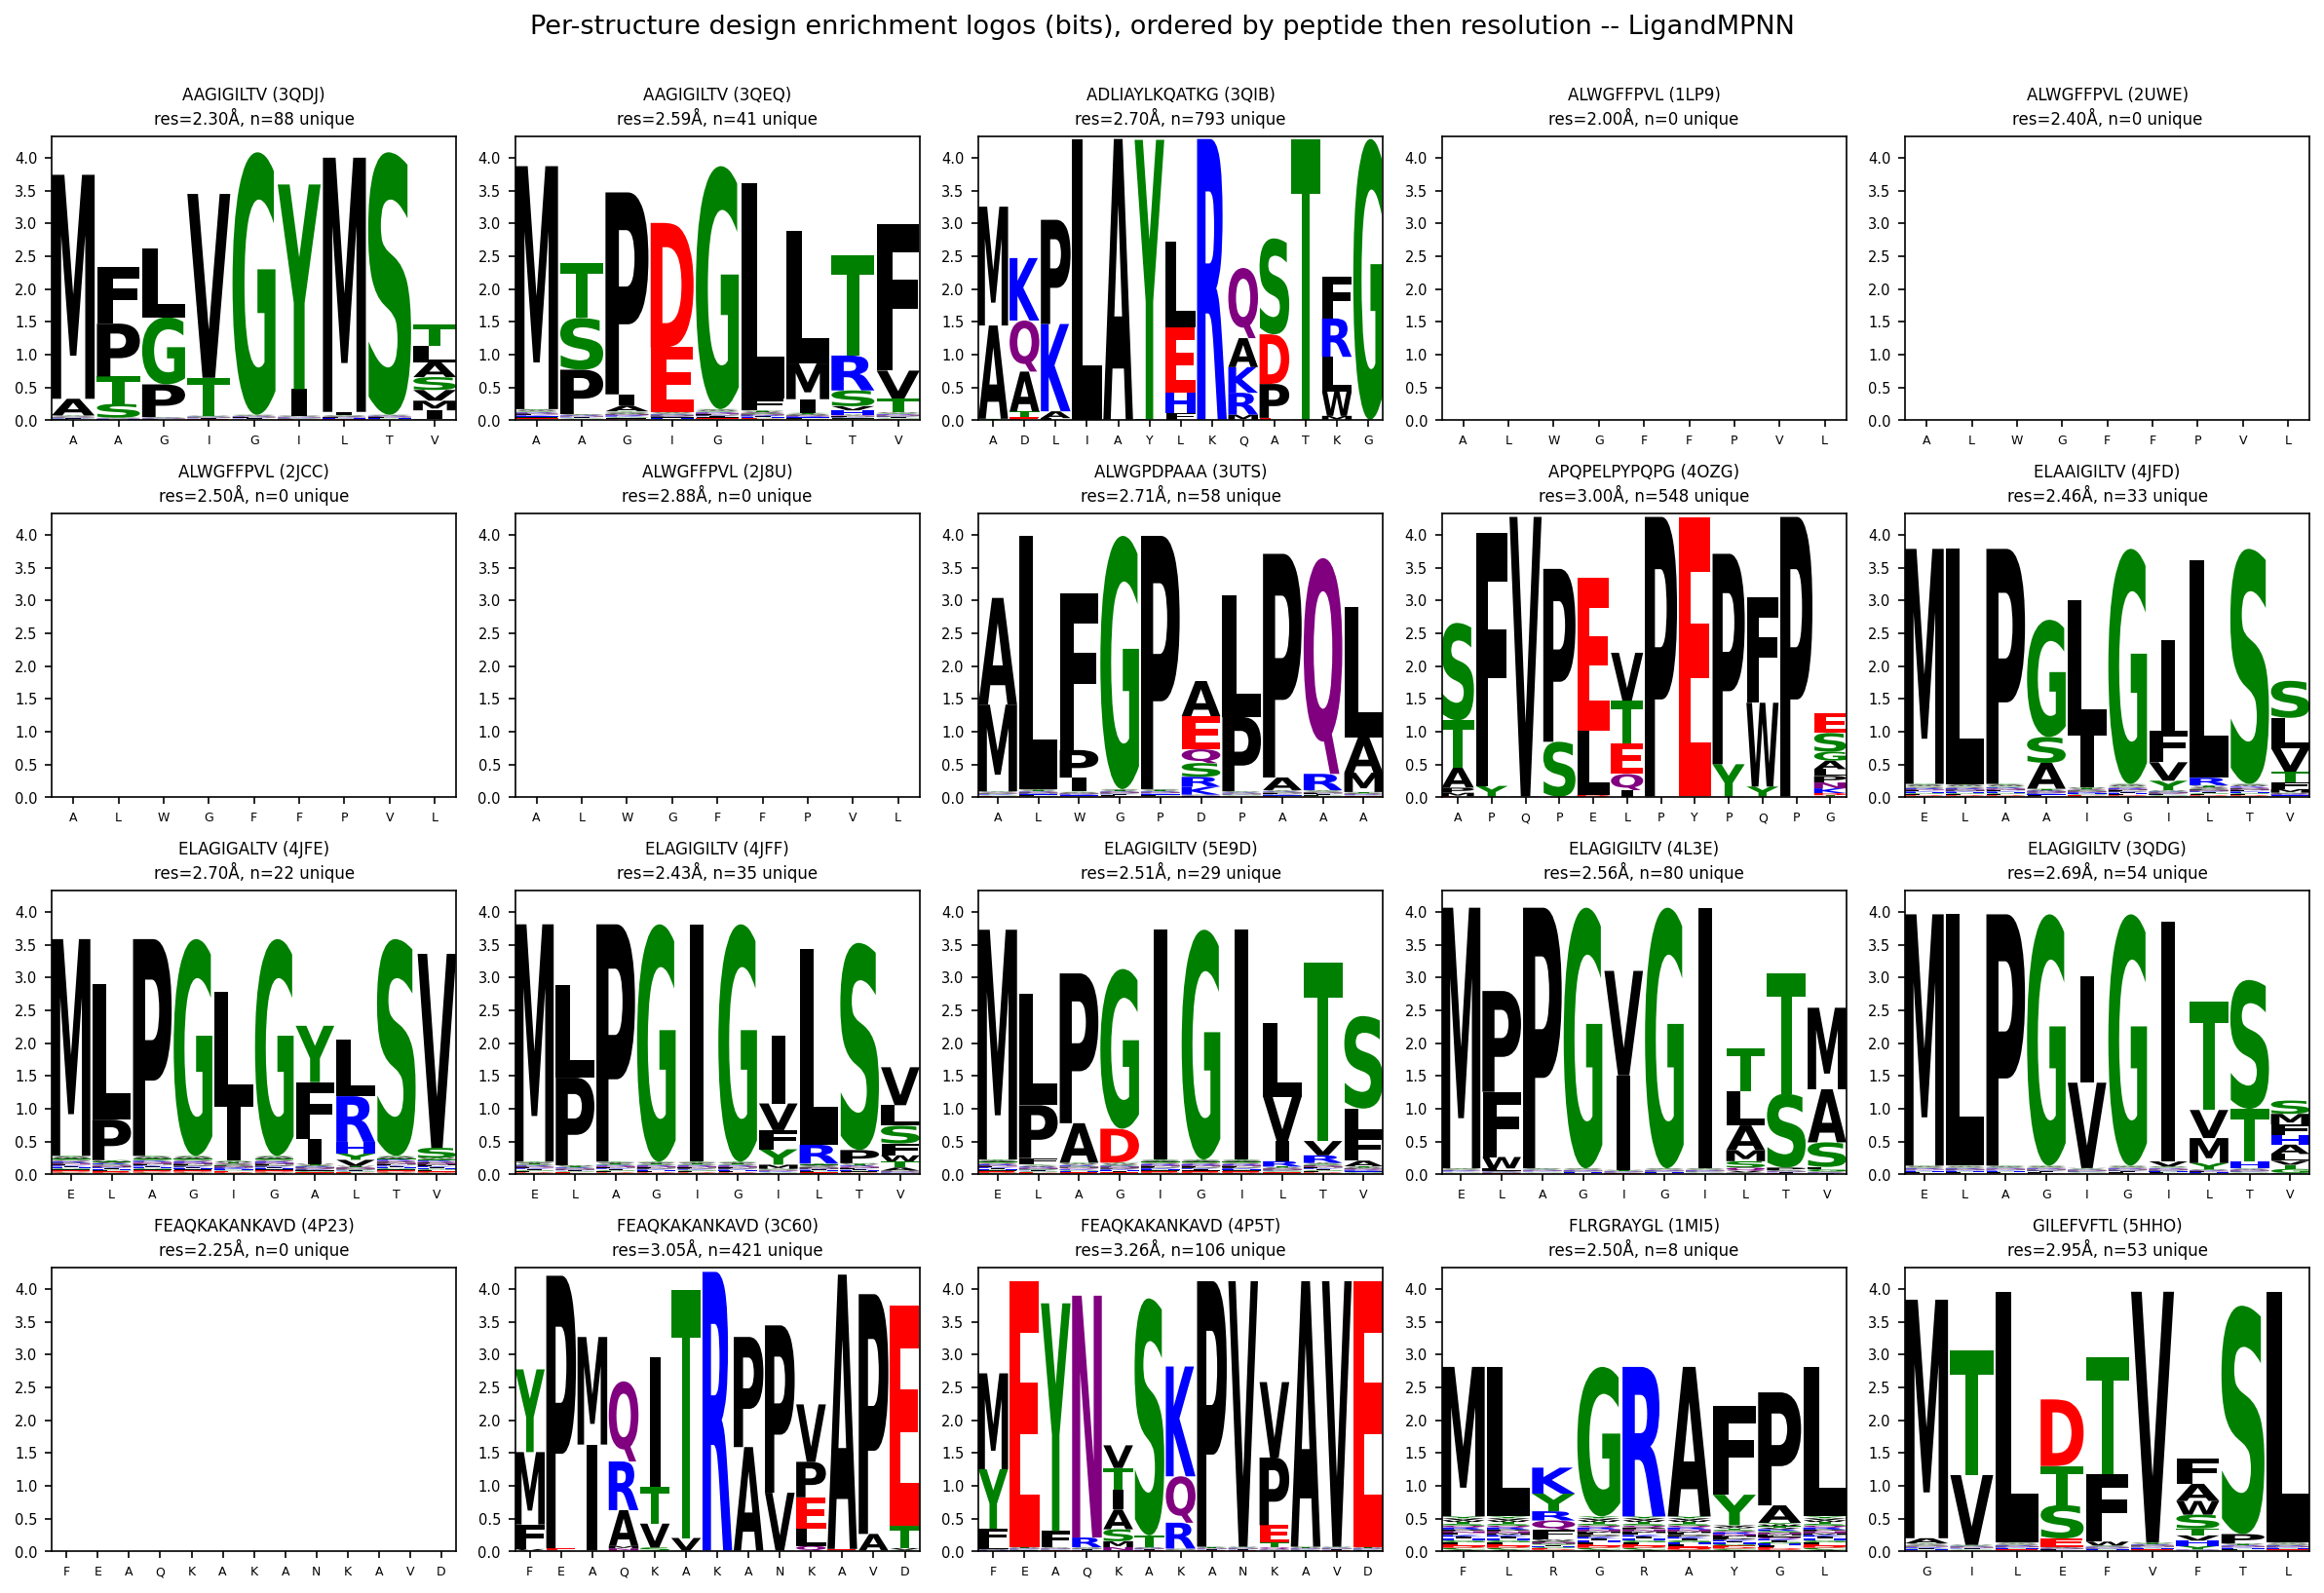
\includegraphics[width=0.7\textwidth]{../figures/fig_panel2_design_presentation/fig_panel2_design_logo_grid_LigandMPNN.png}
\caption{\textbf{Per-structure design logos, LigandMPNN.}}
\label{fig:supp4d}
\end{figure*}

\begin{figure*}[p]
\renewcommand{\thefigure}{S5}
\centering
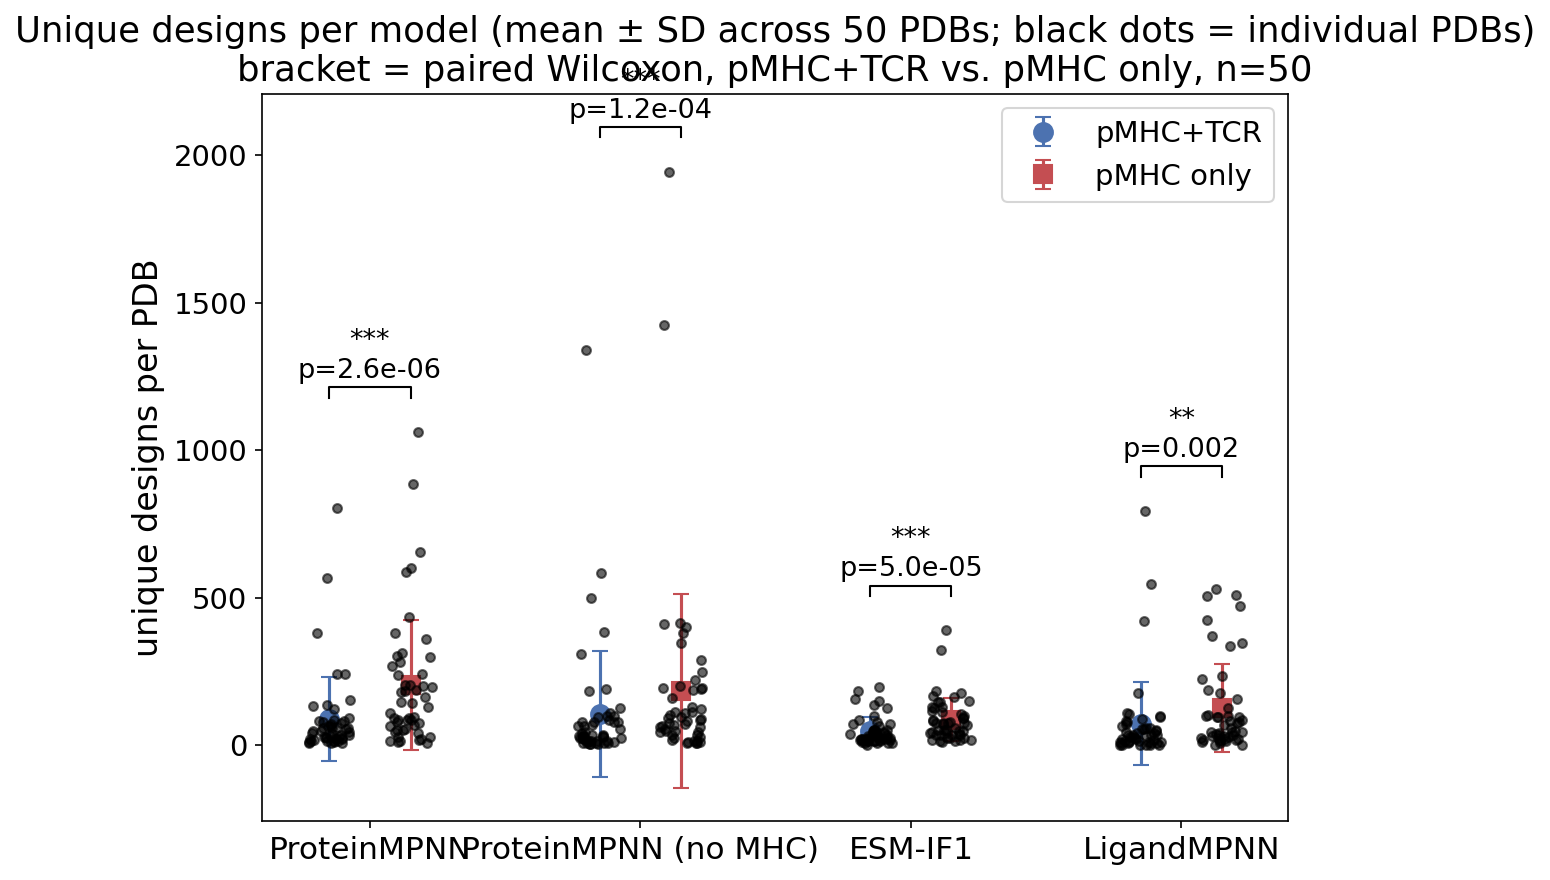
\includegraphics[width=0.75\textwidth]{../figures/fig_panel2_design_presentation/fig_panel2_unique_per_model_meanstd.png}
\caption{\textbf{Unique designs per model, mean $\pm$ SD across structures,}
pMHC+TCR vs.\ pMHC only.}
\label{fig:supp5}
\end{figure*}

\begin{figure*}[p]
\renewcommand{\thefigure}{S6}
\centering
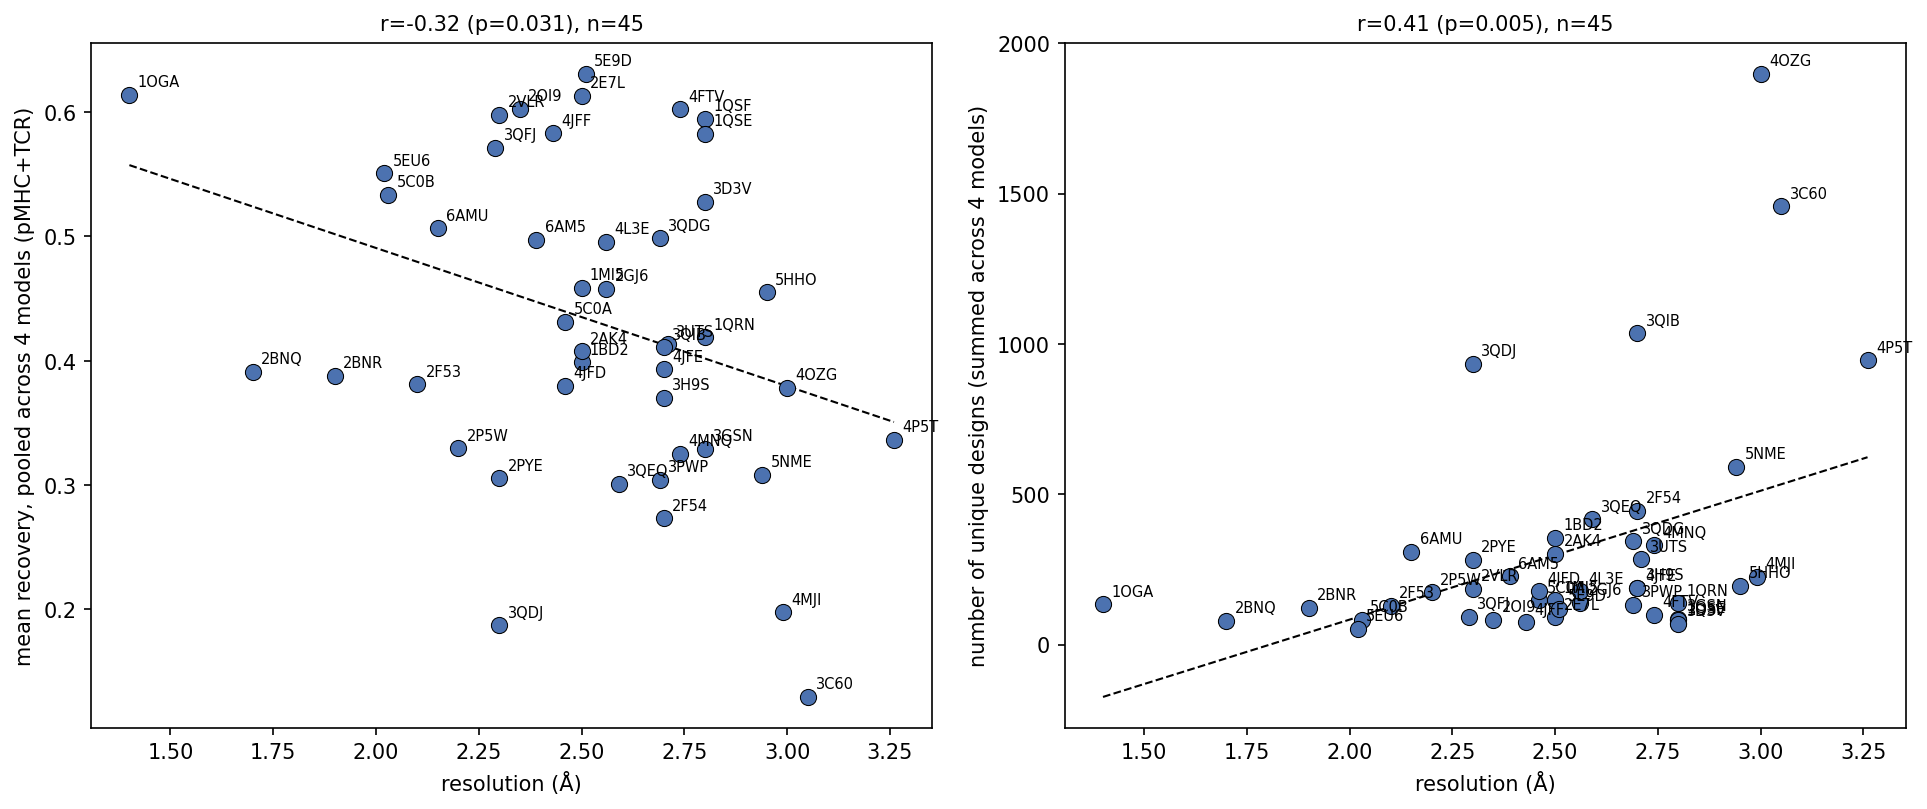
\includegraphics[width=0.75\textwidth]{../figures/fig_panel3_recovery_presentation/fig_panel3_recovery_vs_resolution_and_unique.png}
\caption{\textbf{Resolution and unique-design count vs.\ mean recovery, pooled
across the full 20-structure panel.} $r=-0.49$ ($p=0.030$) and $r=0.45$ ($p=0.049$), $n=20$.}
\label{fig:supp6}
\end{figure*}

\begin{figure*}[p]
\renewcommand{\thefigure}{S7}
\centering
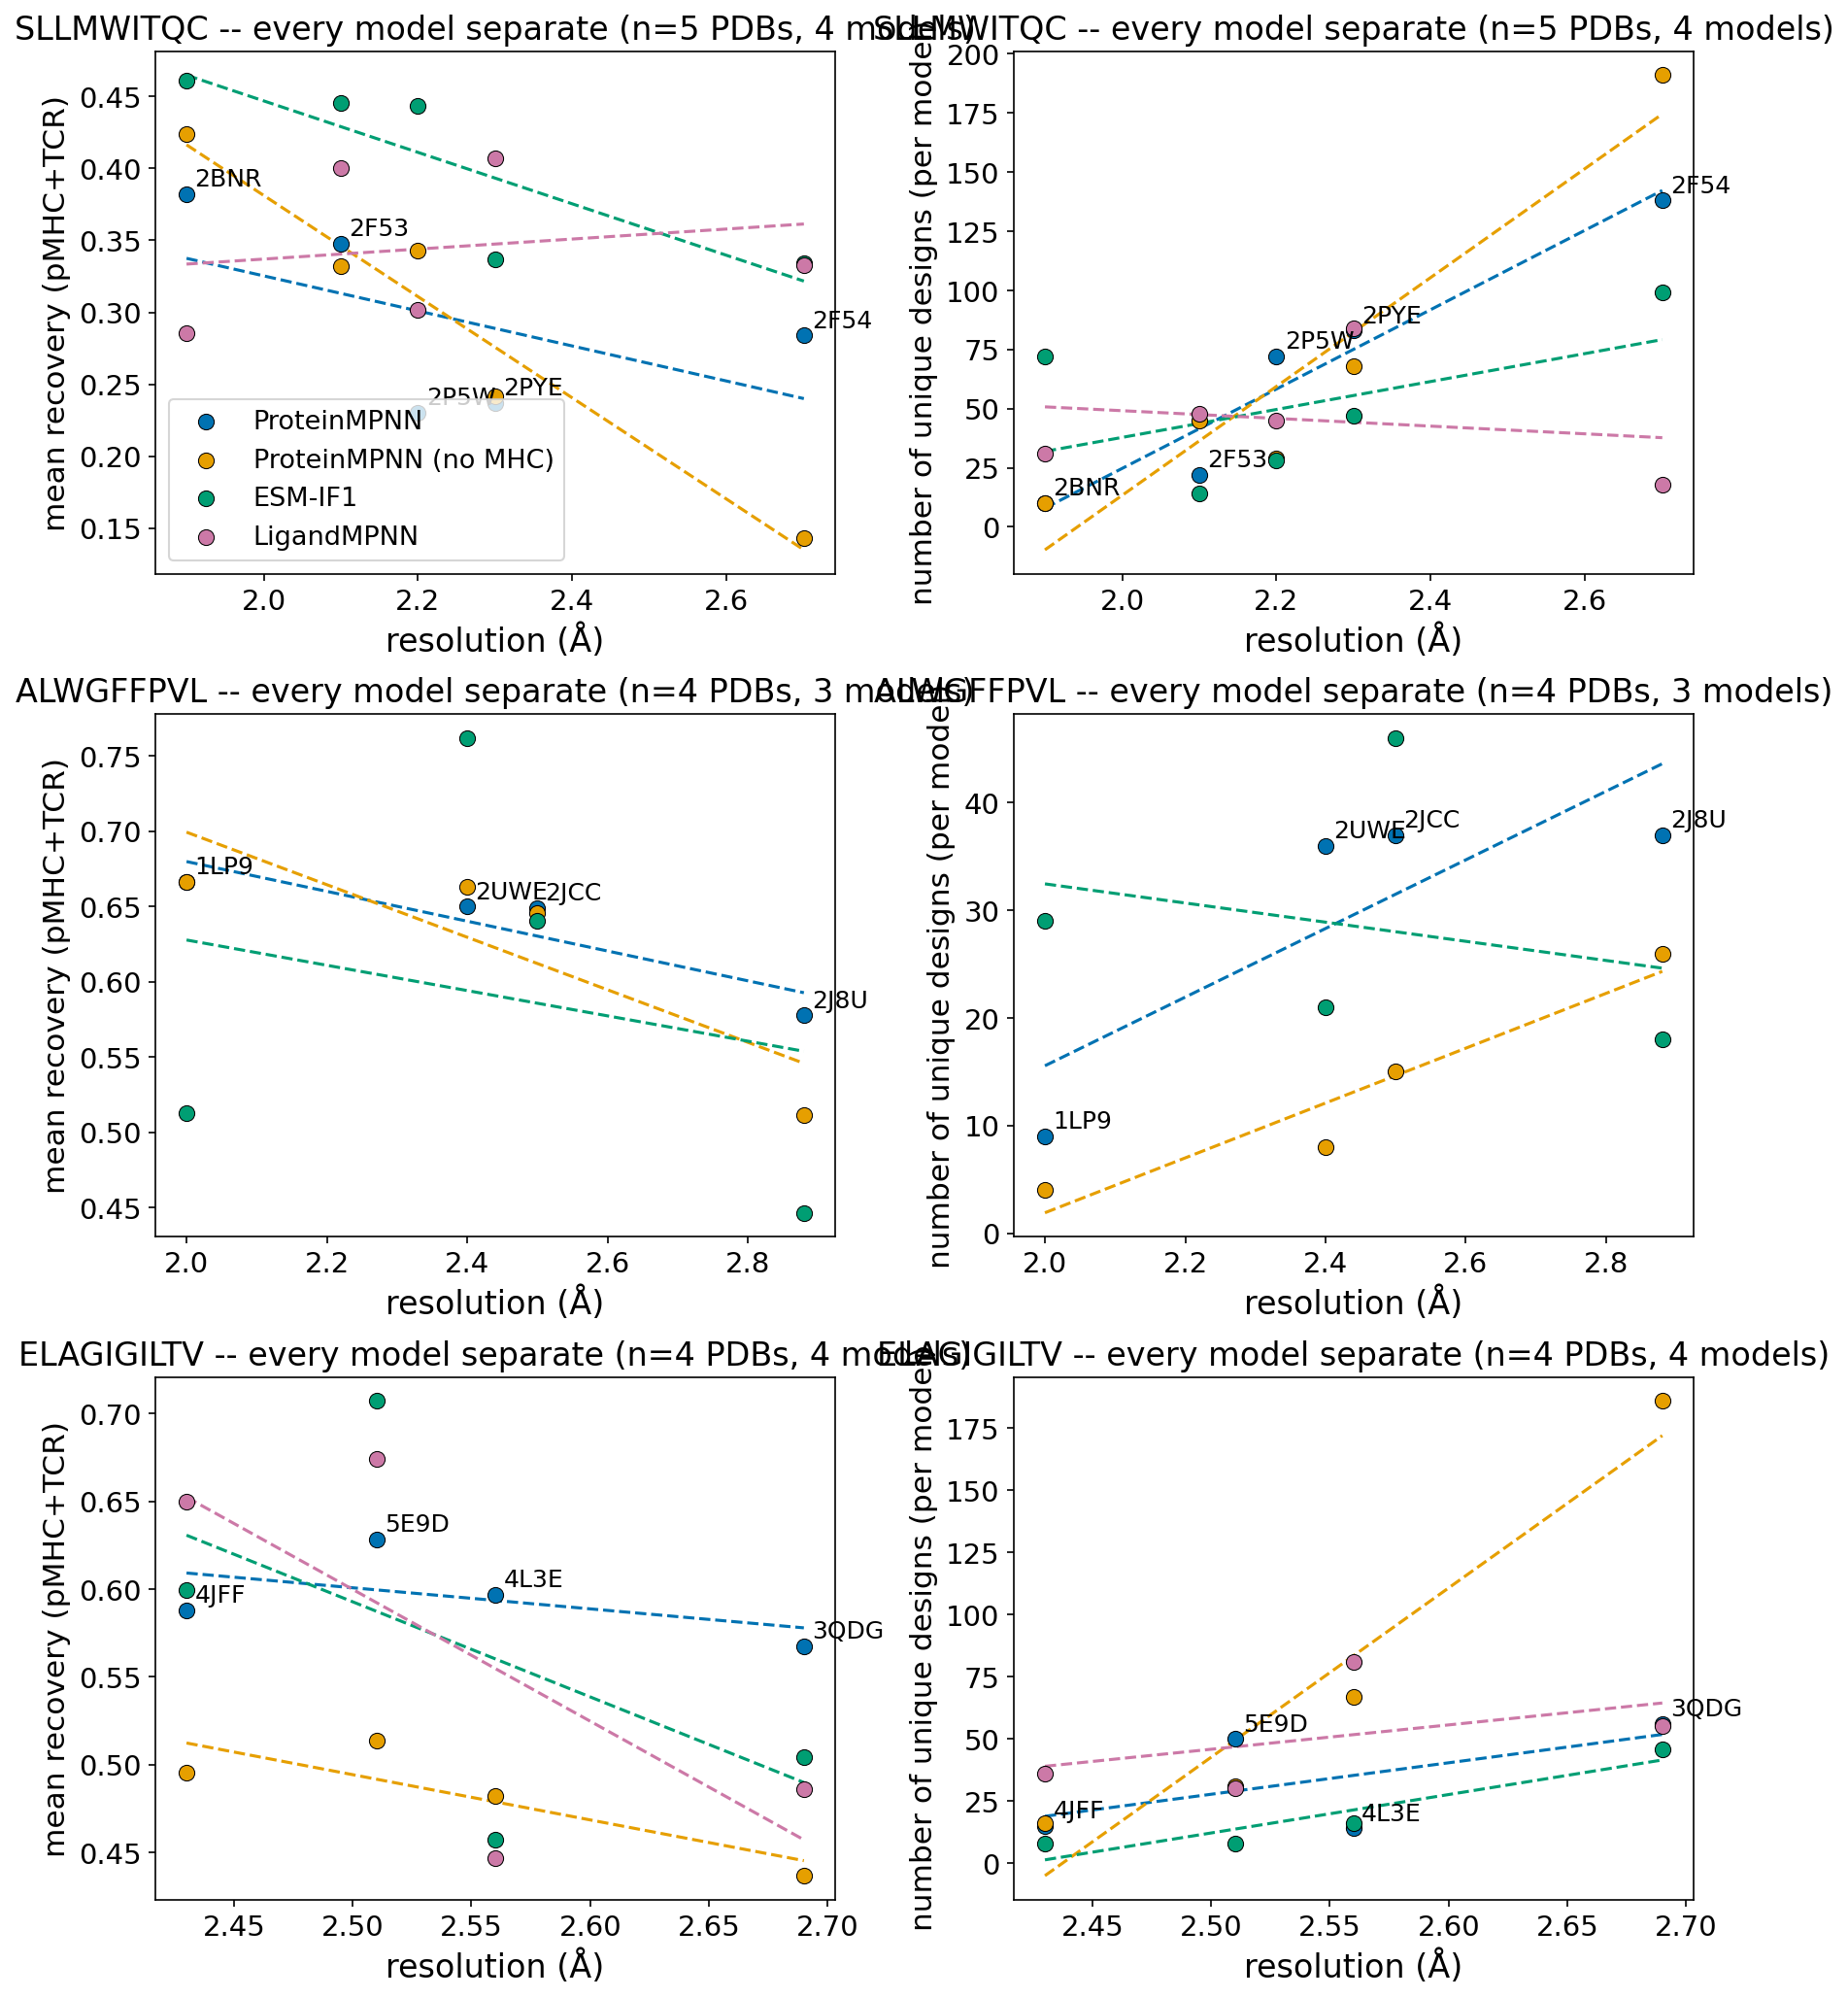
\includegraphics[width=0.75\textwidth]{../figures/fig_panel4_replicate_structures/fig_panel4_full_panel_recovery_vs_quality.png}
\caption{\textbf{Resolution dependence in a controlled, same-peptide replicate
set.} Four structures (2P5W, 2BNR, 2F53, 2F54), identical native peptide, near-identical TCR clone; every
model plotted separately.}
\label{fig:supp7}
\end{figure*}

\begin{figure*}[p]
\renewcommand{\thefigure}{S8a}
\centering
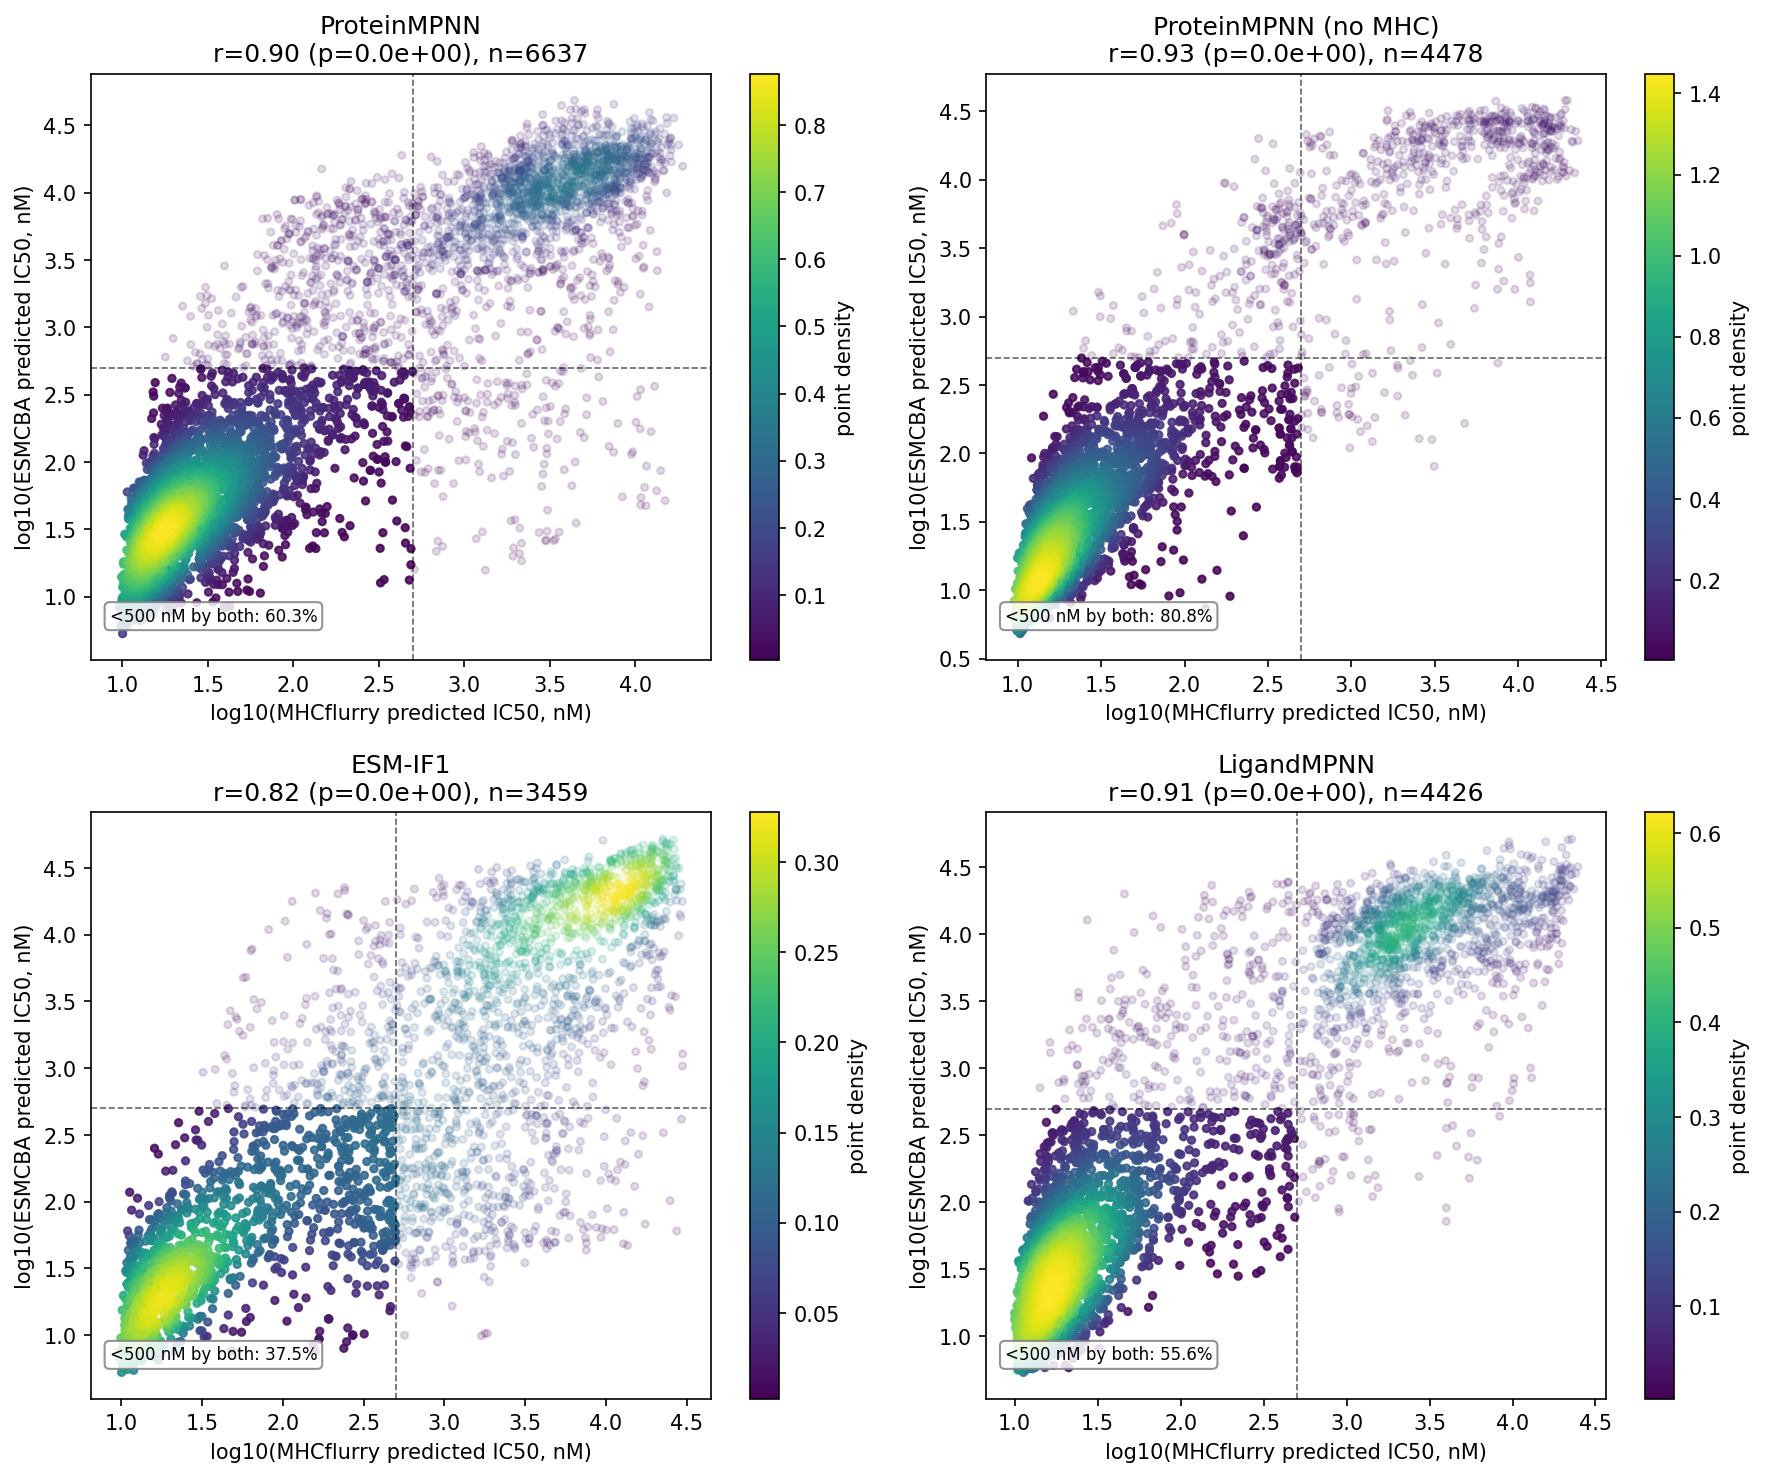
\includegraphics[width=0.75\textwidth]{../figures/fig_panel6_mhcflurry_esmcba_umap/fig_panel6_esmcba_vs_mhcflurry_by_model_mhconly.png}
\caption{\textbf{ESMCBA vs.\ MHCflurry agreement, pMHC-only designs,}
by model.}
\label{fig:supp8a}
\end{figure*}

\begin{figure*}[p]
\renewcommand{\thefigure}{S8b}
\centering
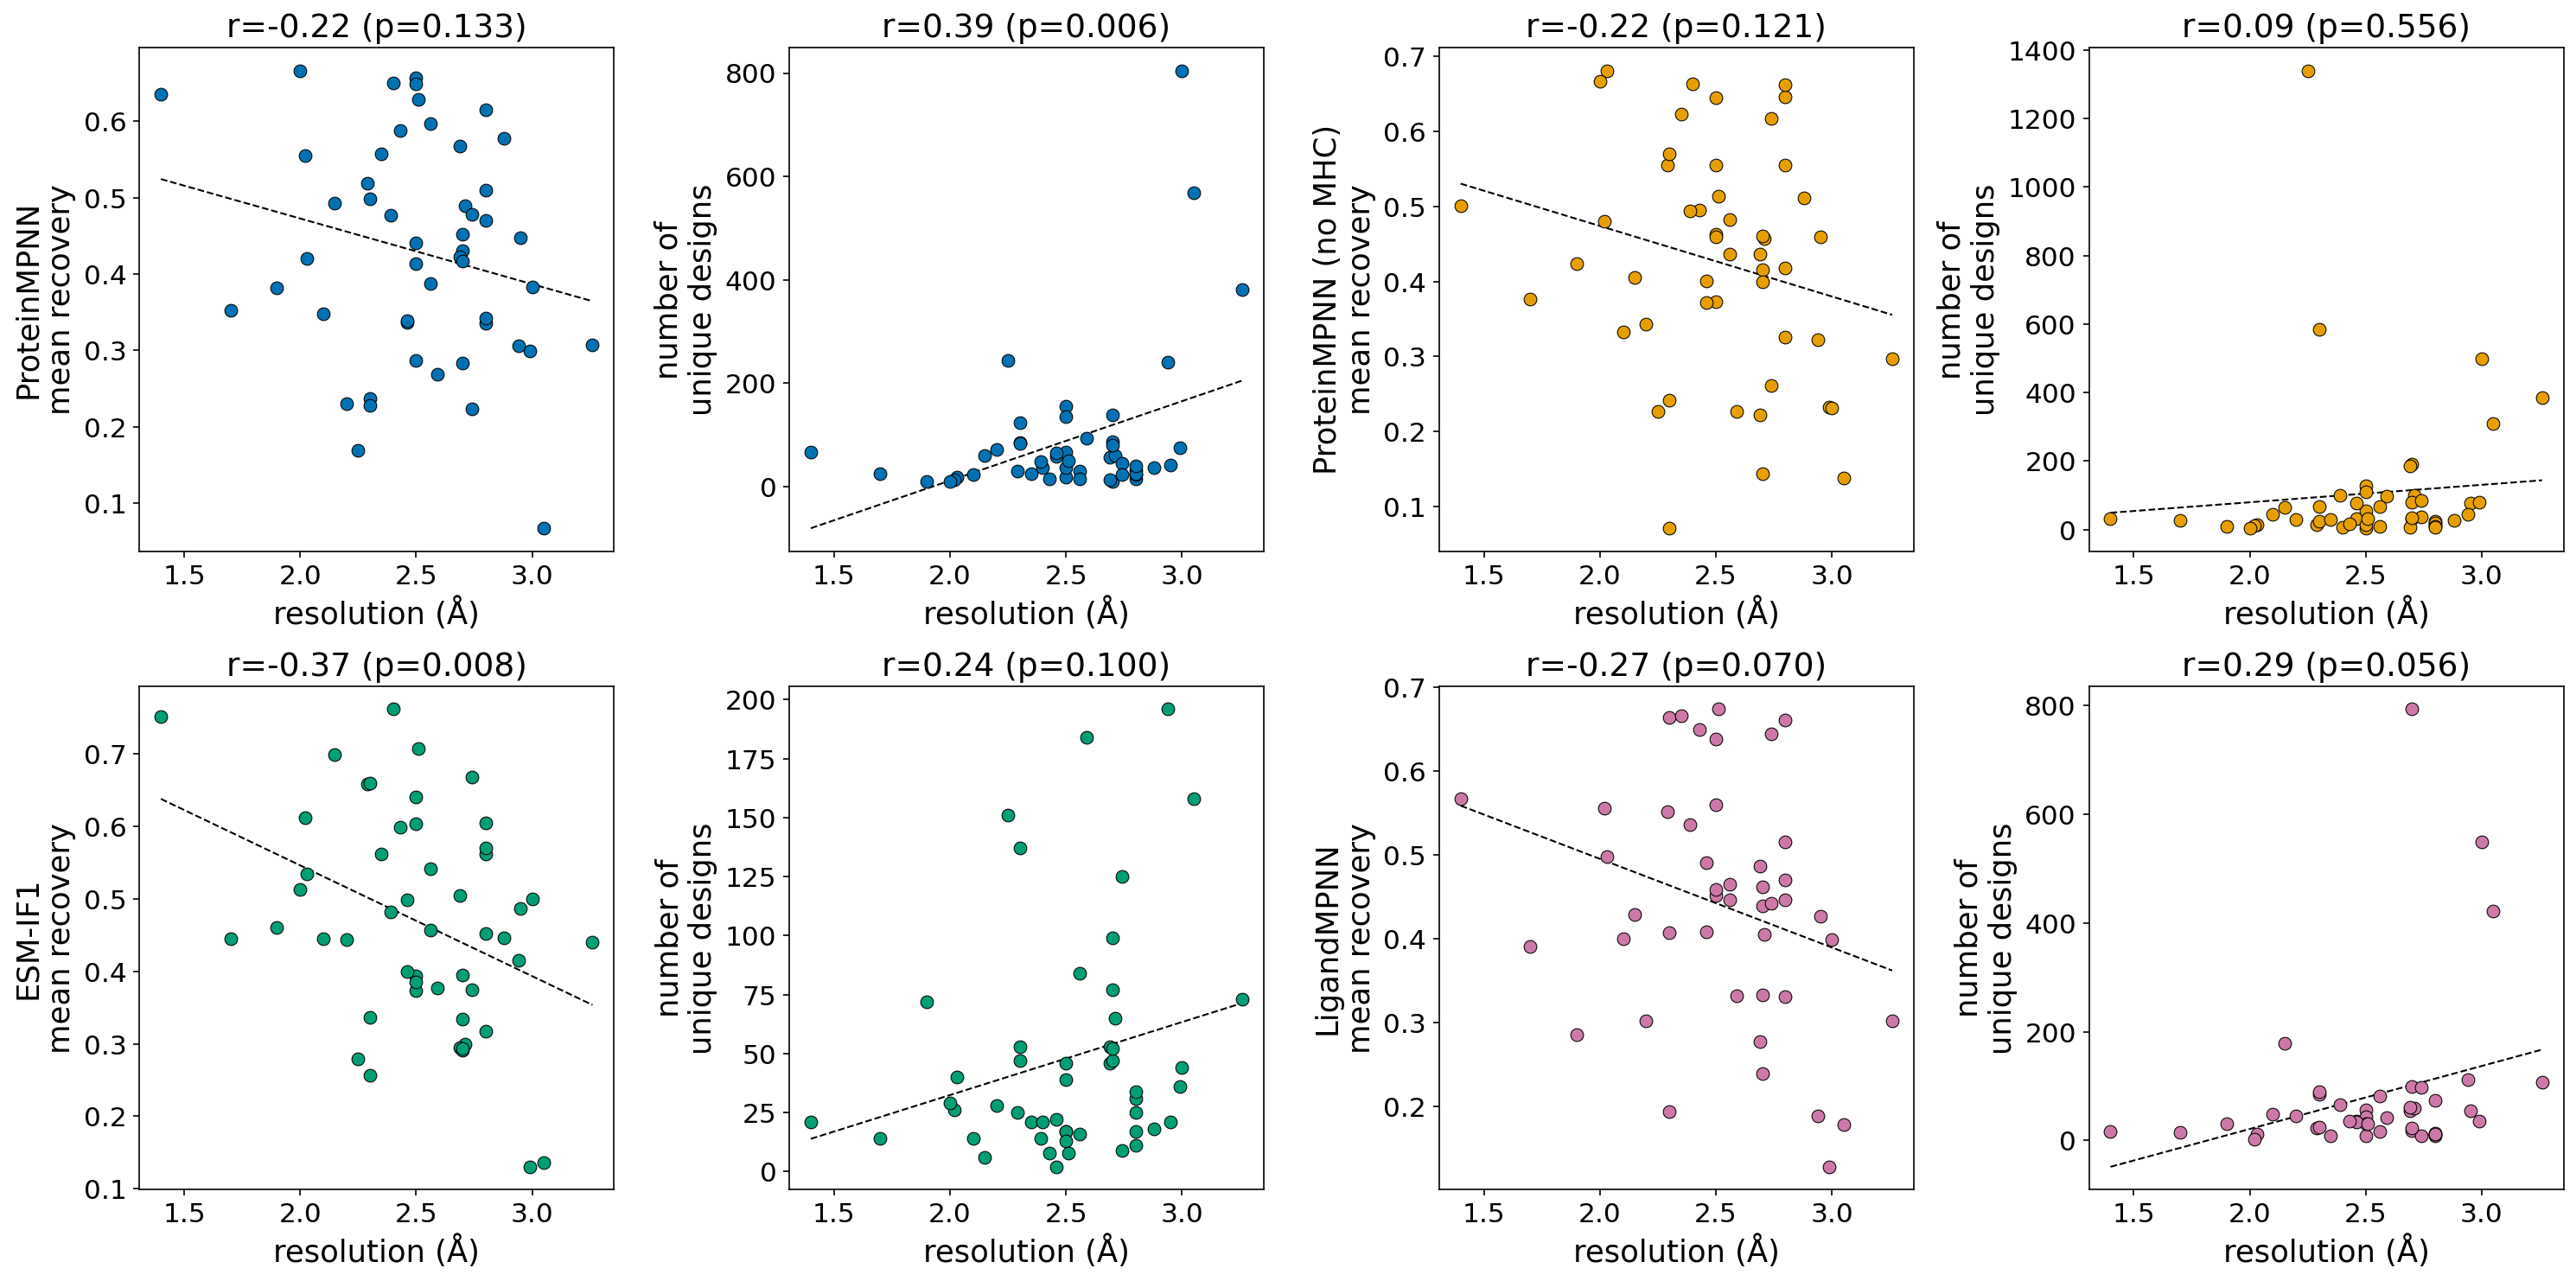
\includegraphics[width=0.75\textwidth]{../figures/fig_panel3_recovery_presentation/fig_panel3_recovery_vs_resolution_and_unique_by_model.png}
\caption{\textbf{Per-model resolution/design-count relationship,} full panel.}
\label{fig:supp8b}
\end{figure*}

\begin{figure*}[p]
\renewcommand{\thefigure}{S9a}
\centering
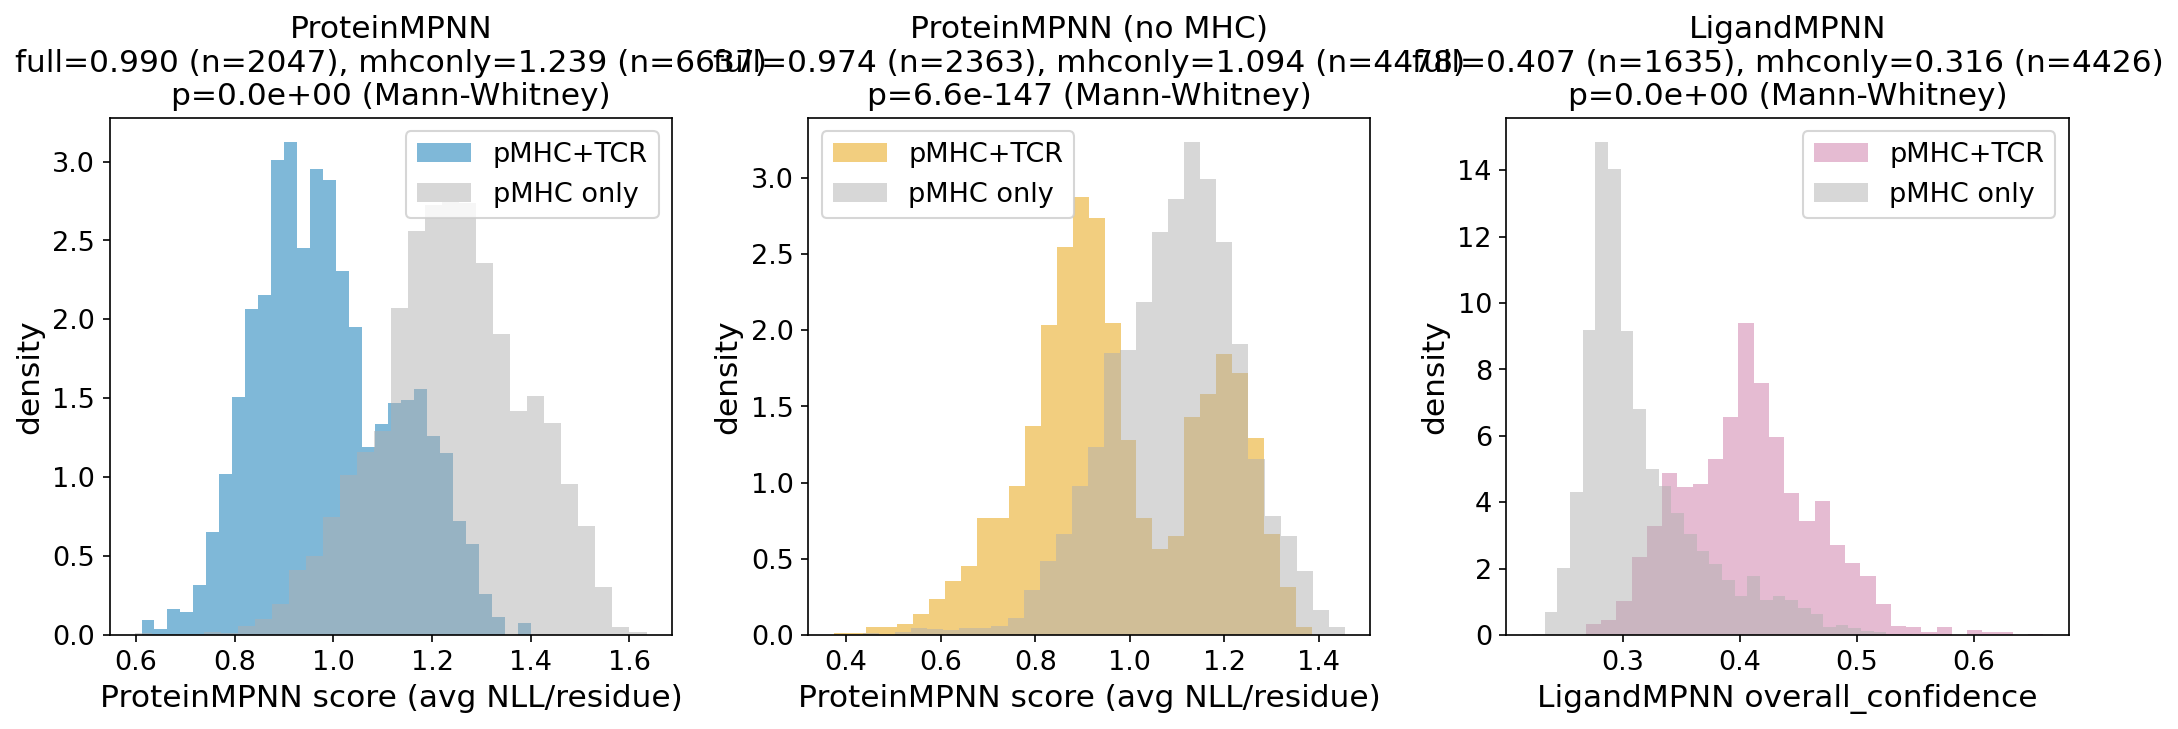
\includegraphics[width=0.85\textwidth]{../figures/fig_panel6_mhcflurry_esmcba_umap/fig_panel6_own_score_shift_pooled.png}
\caption{\textbf{Each model's own confidence score for its designs shifts when
the TCR is removed,} pooled across all nineteen HLA-A*02:01 structures. ProteinMPNN and ProteinMPNN (no
MHC): average per-residue negative log-likelihood, lower is more confident. LigandMPNN: overall
confidence, higher is more confident. All three shift toward lower self-assessed confidence without the
TCR (Mann-Whitney $p<10^{-200}$ in all three cases).}
\label{fig:supp9a}
\end{figure*}

\begin{figure*}[p]
\renewcommand{\thefigure}{S9b}
\centering
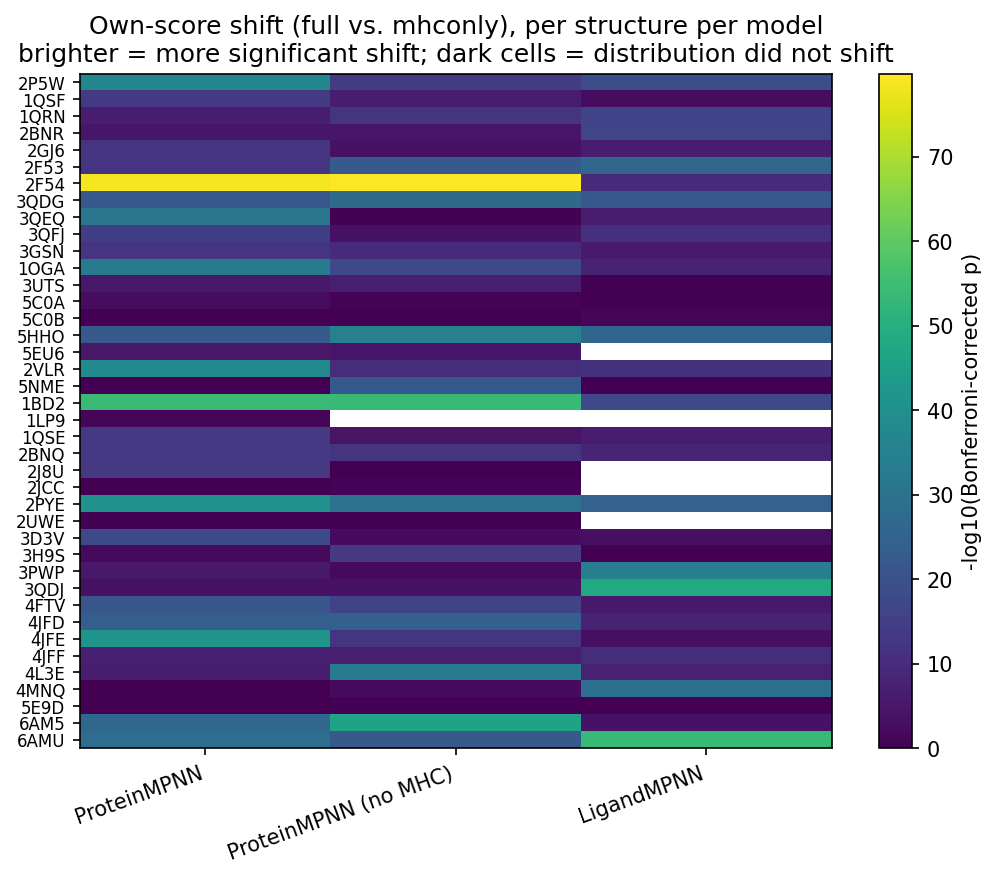
\includegraphics[width=0.7\textwidth]{../figures/fig_panel6_mhcflurry_esmcba_umap/fig_panel6_own_score_shift_by_structure.png}
\caption{\textbf{The own-score shift is not uniform across the panel.}
Bonferroni-corrected significance (full vs.\ mhconly) per structure per model; dark cells are structures
where the model's own-score distribution did not shift.}
\label{fig:supp9b}
\end{figure*}

\begin{figure*}[p]
\renewcommand{\thefigure}{S10}
\centering
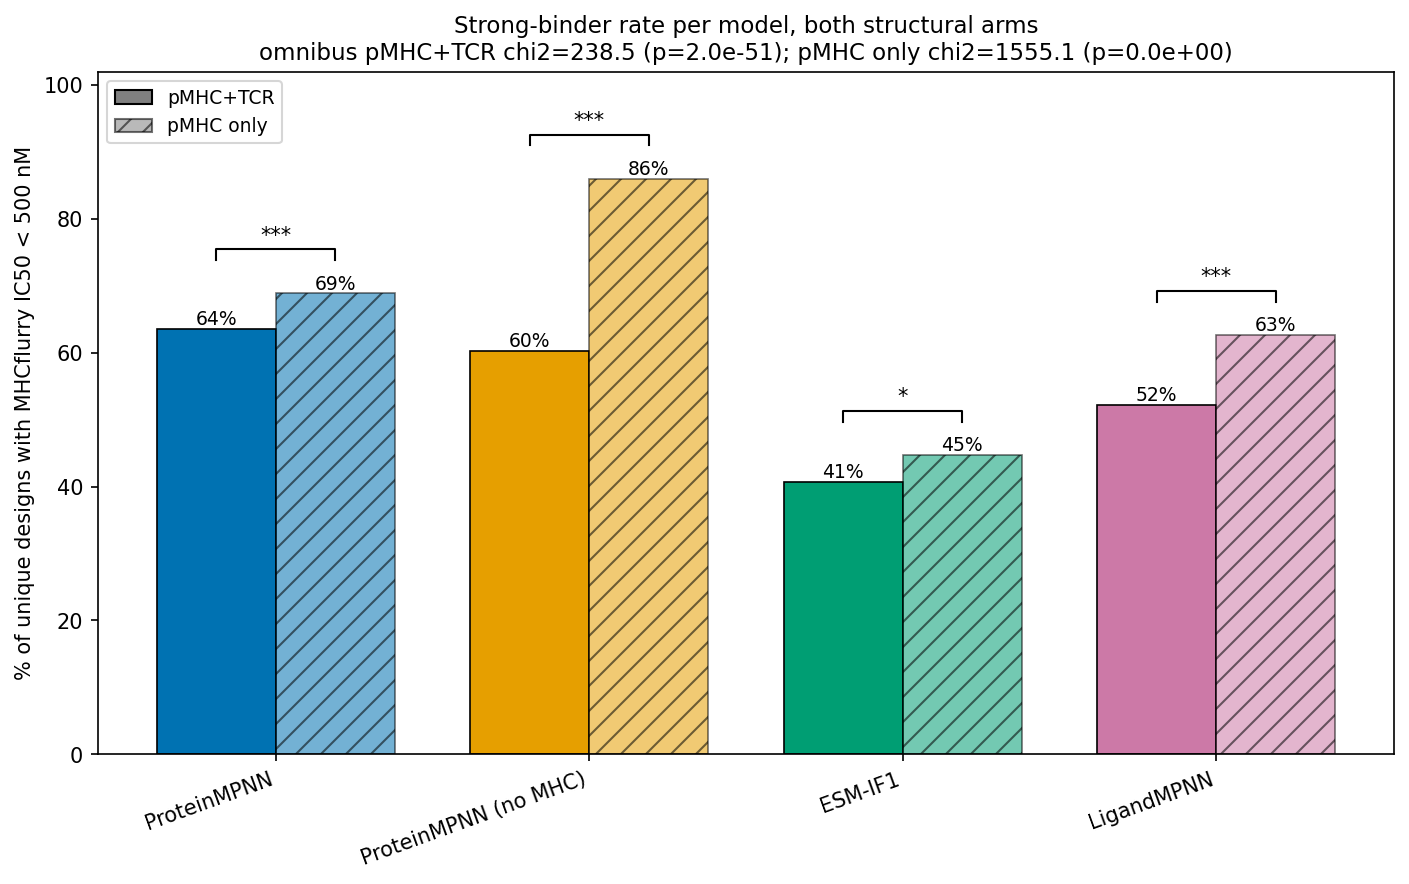
\includegraphics[width=0.75\textwidth]{../figures/fig_panel6_mhcflurry_esmcba_umap/fig_panel6_strong_binder_rate_by_model.png}
\caption{\textbf{Removing the TCR raises predicted affinity, mostly for two of
the four models.} Strong-binder rate (MHCflurry IC50 $<$ 500\,nM), full vs.\ pMHC-only context, Wilson
95\% CI. ProteinMPNN (no MHC) and LigandMPNN both shift up substantially without the TCR; ProteinMPNN
and ESM-IF1 barely move. ESM-IF1 is the lowest-affinity model in both conditions.}
\label{fig:supp10}
\end{figure*}

\begin{figure*}[p]
\renewcommand{\thefigure}{S11}
\centering
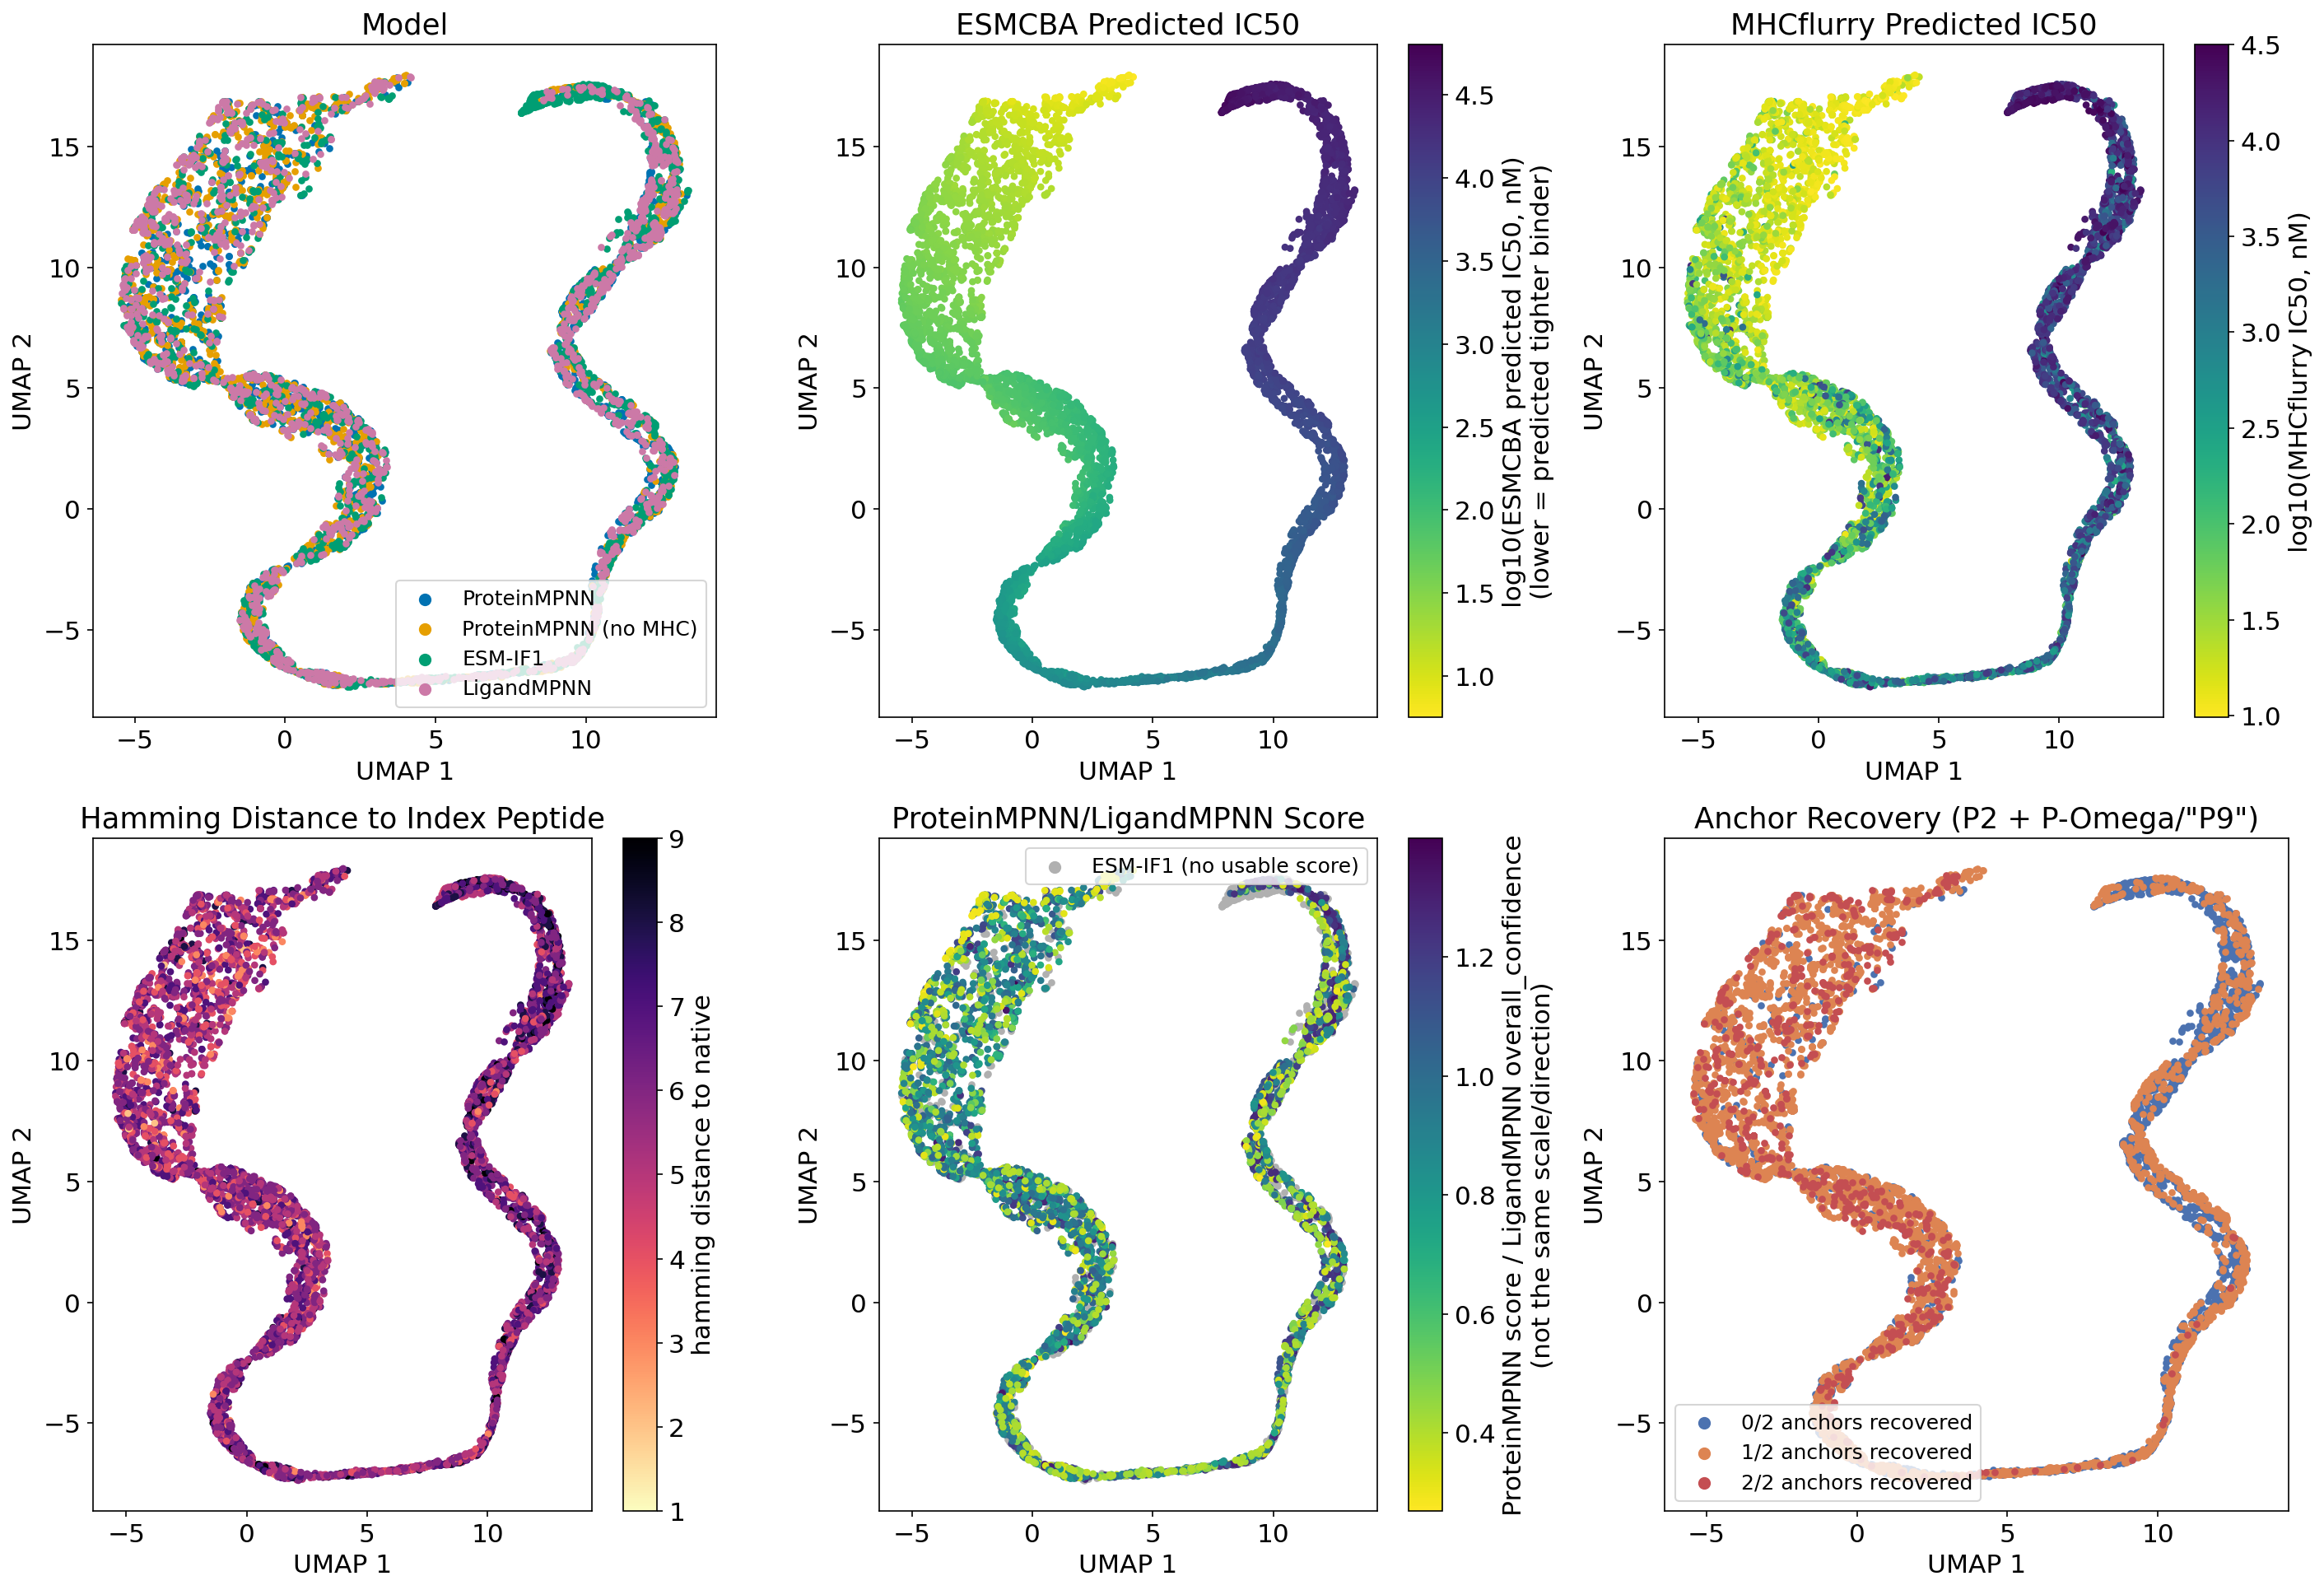
\includegraphics[width=\textwidth]{../figures/fig_panel6_mhcflurry_esmcba_umap/fig_panel6_umap_2x3.png}
\caption{\textbf{The sampled sequence space, colored by predicted binding
affinity.} One UMAP (ESMCBA embeddings, fit jointly over every unique design), recolored six ways. All
four models occupy the same overlapping landscape rather than four separate clusters, and MHCflurry and
ESMCBA, built differently and trained differently, trace the identical gradient across it.}
\label{fig:supp11}
\end{figure*}

\begin{figure*}[p]
\renewcommand{\thefigure}{S12}
\centering
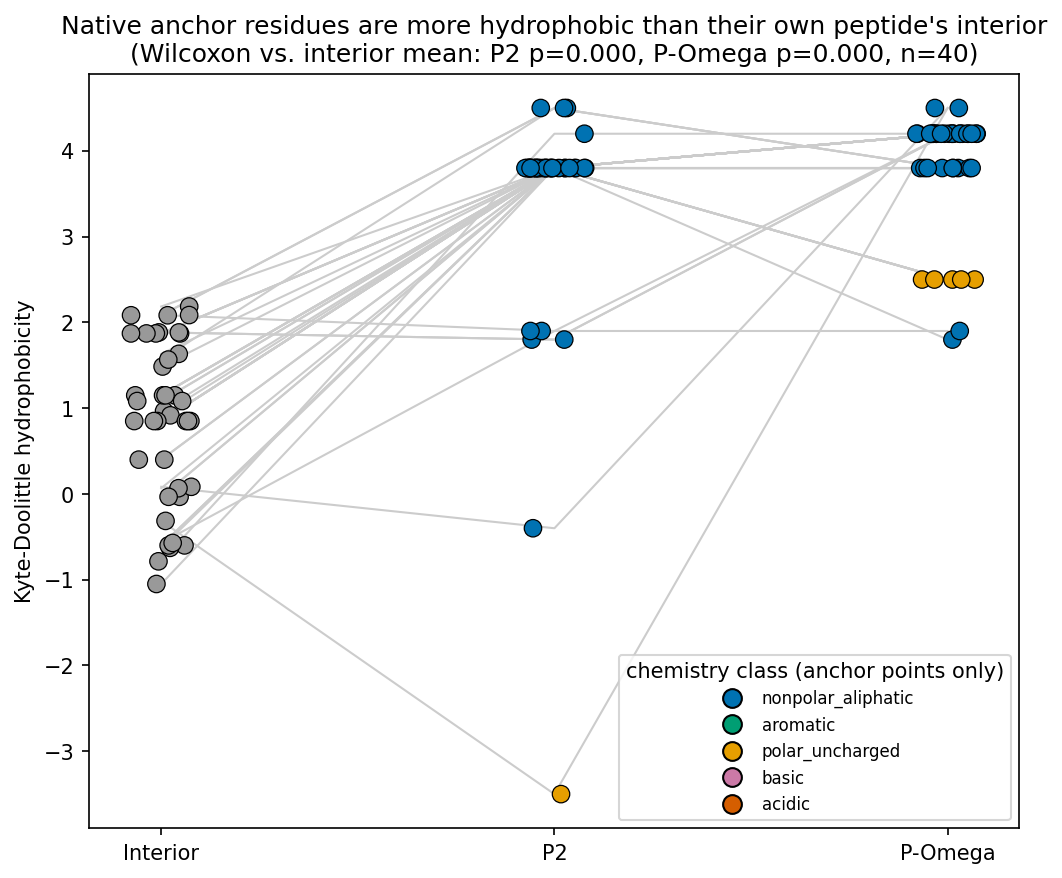
\includegraphics[width=0.62\textwidth]{../figures/fig_panel7_chemistry/fig_panel7_native_anchor_hydrophobicity.png}
\caption{\textbf{Both MHC anchors are more hydrophobic than the peptide interior they sit alongside.}
Kyte-Doolittle hydrophobicity of the native residue at P2 and P$\Omega$ for each of the 19 HLA-A*02:01
structures, plotted against that same peptide's mean over its own interior positions (P3 through the
second-to-last, excluding P1). Grey lines connect the three values belonging to one peptide; anchor
points are colored by side-chain class. Both anchors sit well above their own interior
(paired Wilcoxon, $p=0.0013$ for P2 and $p=0.0001$ for P$\Omega$, $n=19$), so the two pockets do not
differ in whether they prefer hydrophobic residues. They differ in how strictly the designs honor that
preference, which is the distinction reported in Section~\ref{sec:recovery}. The four points at
P$\Omega$ colored as polar are the cysteine-terminated SLLMWITQC/NY-ESO-1 replicates, a residue whose
discrete classification understates its hydrophobicity.}
\label{fig:supp12}
\end{figure*}

\section*{References}

\noindent Ribeiro-Filho, H.V., Jara, G.E., Guerra, J.V.S., Cheung, M., Felbinger, N.R., Pereira, J.G.C.,
Pierce, B.G., and Lopes-de-Oliveira, P.S. 2024. Exploring the potential of structure-based deep learning
approaches for T cell receptor design. \textit{PLOS Computational Biology}.
\url{https://doi.org/10.1371/journal.pcbi.1012489}

\end{document}
